%%%%%%%%%%%%%%%%%%%%%%%%%%%%%%%%%%%%%%%%%%%%%%%%%%%%%%%%%%%%%%%%%%%%%%%%%%%%%%%%
%2345678901234567890123456789012345678901234567890123456789012345678901234567890
%        1         2         3         4         5         6         7         8

\documentclass[letterpaper, 10 pt, conference]{ieeeconf}  % Comment this line out if you need a4paper

%\documentclass[a4paper, 10pt, conference]{ieeeconf}      % Use this line for a4

https://www.overleaf.com/project/5bd3068d4d648d0e5a8b25ad
\IEEEoverridecommandlockouts                              % This command is only needed if 
                                                          % you want to use the \thanks command

\overrideIEEEmargins                                      % Needed to meet printer requirements.

% See the \addtolength command later in the file to balance the column lengths
% on the last page of the document

% The following packages can be found on http:\\www.ctan.org
%\usepackage{graphics} % for pdf, bitmapped graphics files
%\usepackage{epsfig} % for postscript graphics files
%\usepackage{mathptmx} % assumes new font selection scheme installed
%\usepackage{times} % assumes new font selection scheme installed
%\usepackage{amsmath} % assumes amsmath package installed
%\usepackage{amssymb}  % assumes amsmath package installed

\title{\LARGE \bf
 Lab Experiment Subject Management Hybrid Application
}


\author{\IEEEauthorblockN{{Kim bosung}}
\IEEauthorblockA{\\Information System Dept. \\College of Engineering\\
Hanyang Univ\\
Seoul, Korea REP.\\
bosung2697@gmail.com}\and
\IEEEauthorblockN{Nam yunwoo}
\IEEauthorblockA{\\Information System Dept. \\College of Engineering\\
Hanyang Univ\\
Seoul, Korea REP.\\
kikis93@naver.com}\and
\IEEEauthorblockN{Jeong Sujin}
\IEEauthorblockA{\\Information System Dept. \\College of Engineering\\
Hanyang Univ\\
Seoul, Korea REP.\\
wjdtnwls1011@gmail.com}\and
\IEEEauthorblockN{Ha Dongsu}
\IEEauthorblockA{\\Information System Dept. \\College of Engineering\\
Hanyang Univ\\
Seoul, Korea REP.\\
gkehdtn4218@hanmail.net}\and\\
\IEEEauthorblockN{Kim Eunhye}
\IEEauthorblockA{\\Information System Dept. \\College of Engineering\\
Hanyang Univ\\
Seoul, Korea REP.\\
gracekim510@naver.com}
}



\usepackage[utf8]{inputenc}
\usepackage[english]{babel}
\usepackage{graphicx}
\usepackage{tabularx}
\usepackage{tikz-uml}
\usepackage{supertabular}
\begin{document}


\maketitle
\thispagestyle{empty}
\pagestyle{plain}


%%%%%%%%%%%%%%%%%%%%%%%%%%%%%%%%%%%%%%%%%%%%%%%%%%%%%%%%%%%%%%%%%%%%%%%%%%%%%%%%
\begin{abstract}

Lab Experiment Subject Management Hybrid Applicaion (LESM) provides online community where laboratories can post their experiment subject recruitment notices. For the people who are hoping to participate as a subject in a experiment, they can simply find and search for experiments that are suitable and apply for them. 
Using Clinical Subject Management(LESM), laboratories can easily find people they need for experiment and collect sufficient data from experiments. For applicants, they can earn a substantial amount of allowance that laboratories pay for them. Additionally, LESM offers data management service for laboratories. They can figure out their experiment schedule at a glance. Subjects' information will be saved at database server so that laboratories can find a specific data with key information of subjects. By using LESM, laboratories will be able to handle bunch of experiment schedule and result data in a well organized form.\\

\end{abstract}


%%%%%%%%%%%%%%%%%%%%%%%%%%%%%%%%%%%%%%%%%%%%%%%%%%%%%%%%%%%%%%%%%%%%%%%%%%%%%%%%
\maketitle{\textit{Role Assignment\\}}
\maketitle{\textbf{Kim Bosung}}
\subsubsection{Role} Software Developer
\subsubsection{Task description and etc.}
His main job is to create layout of the whole process of development and setting the database. \\
\maketitle{\textbf{Nam Yunwoo}}
\subsubsection{Role} Software Developer
\subsubsection{Task description and etc.} He handles server setting.\\
\maketitle{\textbf{Jeon Sujin}}
\subsubsection{Role} Development Manager
\subsubsection{Task description and etc.} He checks the flow of development process.\\
\maketitle{\textbf{Ha Dongsu}}
\subsubsection{Role} Software Developer
\subsubsection{Task description and etc.} He designs the front end.\\
\maketitle{\textbf{Kim Eunhye}}
\subsubsection{Role} User/Customer
\subsubsection{Task description and etc.} Contact with potential users and get feedback from them.\\

\section{INTRODUCTION}
\maketitle{\textbf{Motivation\\}}

Because there was no platform that allows communication between laboratories and people, it is hard for laboratories researcher to find clinical subjects. Previously, they had to find subjects through personal ways. For example, they had to make a recruitment notice to print out and post or to upload at small websites. They also had to receive text and reply one by one with their own phone. And researchers had to put all the information about each applicants and schedules from text messages to excel file. So we decided to create a platform that allows the lab to post recruitment notice and students to look at it and apply for what they want. And Because there were no such things that manage their experimental data, we add one more thing in our app. A simple database system. Researchers can keep their test result or subjects’ personal data efficiently. There are a lot of data that researchers want to review afterwards. Since bunch of data are accumulated steadily, they frequently have difficulty finding out the specific information they need without systematic database. By saving all the data related to experiments, it will be a lot easier to handle and search for it. \\

\subsection{Data Transaction\\}

\subsubsection{Previous Way Of Data Transaction}
Applicants provide their personal information via \textbf{text message or e-mail.} 
Researchers save the information in the format of \textbf{excel}. In worse cases,it is saved at their \textbf{phone contact list}\textbf{ or .txt file}.\\
Researchers provide information about experiments via recruitment notice posted at \textbf{school online community} or at \textbf{bulletin board in school buildings}. Applicants have very limited way of obtaining this information because the preferred posting location is different among diverse laboratories. This means that recruitment notices are dispersed. Also, they usually save the experiment information \textbf{by taking a picture or screen shot of the notices.}
Experiment result data is saved at \textbf{researchers personal PC} in the format of excel, .bdf, .mat or word.\\

\subsubsection{\textbf{Data That Applicants Need From Researcher}\\}
\begin{itemize}
\item Name Of Experiment
\item Main Purpose Of Experiment
\item Location
\item Date and Time 
\item Expected Duration Time
\item Specific Process Of Experiment
\item Payment
\item Condition For The Adequate Subjects\\
\end{itemize}



\subsubsection{\textbf{Data That Researchers Need From Applicants\\}}
\begin{itemize}
\item Name
\item Age
\item Sex
\item E-mail Address
\item Contact Number
\item Possible Date and Time\\
\end{itemize}

\subsubsection{\textbf{Result Data That Researchers Get After Experiment\\} }
\begin{itemize}
\item Raw data such as .bdf and .mat
\item Result data of raw data analysis. Such as excel and doc.
\item Special features for each of subjects.\\
\end{itemize}

\subsubsection{\textbf{Data That Researchers Upload To DB\\}}
\begin{itemize}
\item Result data of experiment
\item Name of Lab
\item Experiment types that are held in the lab
\item Name of University(Location)
\item Contact number 
\item Email address
\item Special features for each of subjects
\item Schedule of experiments.
\item Detailed information of experiments for applicants.\\
\end{itemize}

\subsubsection{\textbf{Data That Database Return To Researchers\\} }
\begin{itemize}
\item Subjects personal information who have previously participated
\item Scheduled experiment date
\item Experiment date records
\item Result data of experiment\\
\end{itemize}

\subsection{Data Transaction Efficiency\\}
\maketitle{\textbf{Inefficiency of Data Transaction}\\}
    Fundamentally, the inefficiency is caused by lack of database system between applicants and researchers. 
\begin{itemize}
    \item The recruitment notices are dispersed. Some are posted online and others are printed out to be posted in bulletin board. Like this, there are a number of recruitment notices which are huge volume of data required by people who hope to apply as subject. This inefficiency problem arises since there is no platform that contains these data at a systemized database. Researchers cannot deliver the notice to potential applicants and applicants have no other way but to wander around online community and bulletin board to get the notice information.
    \item When applicants send their personal information via text message or e-mail, researchers have to copy all the information to excel or .txt file by himself. They also have to save the contact number of applicants in their phone since they need to keep in contact for organizing experiment date and time or to discuss about payment. 
    \item Researchers have to handle bunch of data related to experiments. It includes information of applicants and experiment result or date. Researchers do have their on way of organizing and saving these data but it is inefficient without database server. They usually save the data at local drive with custom folder. Then they inevitably have to memorize the folder location, name and the type of data saved in it.  
\end{itemize}



\subsection{\textbf{Software In Use}}


\subsubsection{Albamon}

It is one of the most famous applications for students to search part-time job. It provides information of various jobs. Job seekers can set up your own interests and receive push notifications for that. And they can fill out their resumes to keep it in the app.

\subsubsection{Olive C}
This application makes it easy to provide recent clinical information. People can participate in that clinical test if it’s good for themselves. There are Different things between Olive C and our application. CSM  is only used in Hanyang Lab, and it can database the result of the clinic




\section{REQUIREMENT ANALYSIS\\}


\subsection{Account Management}
\subsubsection{Separate Account Data}
There are two types of users. The lab researchers and applicants for experiments. For each of the user type, different main page will be shown that contains different functions. At the very first page, users have to choose whether they are lab researchers or applicants. 
\subsubsection{Sign Up}
For the lab researcher member, it is required to register the lab and his or her e-mail address. Only one account will be assigned to a lab. For the applicants, they have to enter their e-mail address, name and phone number. This information will be delivered to researchers who manage the experiment that the applicant applies. 
\subsubsection{Log In}
After clicking the check box whether they are lab researchers or applicants at the very first page, log in page will be shown. Users can sign in with their e-mail address and password. 


\subsection{Functions For Lab}

\subsubsection{Main Page}
The experiment schedule of the lab will be shown in the form of calender. Also, the list of experiment instances will be shown with drop down. There is another list that shows all the researcher registered in that lab. The general manger has authority with this list. There is a button for adding new experiment instance to the drop down list. When one of the experiment instances is clicked, sub main page for each experiment will be shown. 
\subsubsection{Sub Main Page For Each Type Of Experiment}
There are three main functions in this page. One for managing the previous data of specific experiment, another for posting recruitment notice and the other for uploading experiment result data. 

%%%%%%%%%%수정하자~ㅜㅜ%%%%%%%%%%%%%
\subsubsection{Reviewing Previous Experiment Reault }
The user can easily search for specific experiment data with subject information like name, age or date of experiment. 
\subsubsection{Uploading/Revising Experiment Result Data}
If a researcher selects one of the experiments in the list and click this button at the main page, the page of uploading and revising for the experiment result data will be shown. The researcher in charge can enter the date,time, explanatory comment, name and other special features of the subject. It is also possible to request for personal information like age and gender. 
\subsubsection{Create Experiment Instance}
After clicking the button for creation of new experiment instance at the main page, pop-up for entering specific information of the new experiment will be shown. Only the general manager can use this function. The name of the researcher in charge, experiment objective and the name and type of the experiment should be entered. 
\subsubsection{Posting the Recruitment Notice}
After clicking the button for posting recruitment notice at the main page, the researcher in charge moves to the next page. In this page, the researcher should make the schedule of the experiment date and time via calender UI. Then the researcher should enter the specific information like the payment, condition, the method of experiment, place of the laboratory, expected duration time. The notice form delivered to the applicants page will automatically include these details in addition to name of the experiment, name of the researcher in charge, date and time. This notice form will be loaded to the applicants' main page.
%%%%%%%%%%%%%%%%%%%%%%%%%%%%%%%%%%%

\subsection{Functions For Applicants}
\subsubsection{Main Page}
In this page, users can see the list of recruitment notices in a similar form like Albamon bulletin board. They can search specific experiment by setting conditions like the type,payment and date. Then the list will be organized in order of payment and deadline.
\subsubsection{Detail Information Page}
If users click one of the recruitment notices, they move to the next page which contains details of the experiment. It shows the information that are entered by the researcher in charge. Additionally, there is a calender. Each date box in the calendar might contain the time of experiment that researcher has scheduled and posted at previous stage. Small message boxes are attached to each of the scheduled date which indicate whether it is fully booked or not.  The applicants can only choose the date that is not full. The applicant should first check one of date boxes and click apply button. This apply button will show pop-up with the message of "successfully applied". Also, as soon as the button is clicked, the message box of that date should be changed to indicate that there is no opening. 
\subsubsection{My Page}
In the main page, users can move to MyPage by clicking the button of 'MyPage'. In this page, they can see a list which contains all the experiments that they have applied for. They can see the brief information such as the name of experiment, location, contact number of researcher and the date they have participated or scheduled to participate. On the left side of each element, there are check boxes. If users want to cancel some of the experiments,they should click the check boxes and then click the 'cancel' button. If they want to see the whole detailed information about a experiment, they should click a element in the list. Then they can move on to the information page.
\subsubsection{Information Page For Experiments In MyPage}
This page will contain all the information of the experiment that applicants have applied for. This will fulfill the need that applicants want to review the specific detail of the experiments they are going to participate afterward.

%%%%%기획에 반영안했지만 그래도 라텍스에는 삭제하지 말고 남겨놓으라 하심
\subsection{Communication Between Applicants and Lab}
\subsubsection{Message Drop Box}
If applicant wants to reschedule or make inquiries, sending direct message will be useful. With this service, the researchers do not need to reply with their own phone or e-mail. 
\subsubsection{Communication page for Lab}
This page shows the list of scheduled experiments. The elements can be divided according to whether there are applicants or not. There is pop-up notice that tell them every time someone apply for the experiment. Also, there is drop box which contain all the inquiry messages from applicant and reply to them. 
\subsubsection{Communication page for Applicants}
After clicking the inquiry message button at the page of detailed information, pop-up will be shown to enter inquiry message. This message will be saved in the account's drop box. 
%%%%%%%%%%

\section{\\DEVELOPMENT ENVIRONMENT}
\subsection{Choice of software development platform}

\maketitle{\textit{Form of application: Hybrid Application}}

We were trying to create an application only. However, we figured out that the application alone is not sufficient for users and the laboratory to write and post a notice. To be specific, the main problem is that the data file which the lab researchers handle is not a simple task. In most cases, the file format is .bdf and .mat. These data files are usually stored at the desktop computer in the lab. If we create mobile application, it will be difficult to deliver the file from local desktop to the server. Additionally, there are a lot of things to type in when posting a notice, entering personal information and so on. Therefore, we decided to make a hybrid application. We will make a web for the laboratory and use reaction type web for the mobile application. 

\maketitle{\textit{Programming Language}}
Additionally, we will use html and css to make web page’s basic and style, and decorate the web page using javascript (javascript 1.8.5), bootstrap and jQuery (jQuery 3.3.1). In the back-end, we will use the PHP with Laravel framework and MySQL to implement the database. 


\begin{supertabular}{ |p{1cm}|p{5cm}|p{1cm}|  }
 \hline
 \multicolumn{3}{|c|}{Tools} \\
 \hline
 Cordova Adobe Phonegap& In order to develop the hybrid application, we decided to use Cordova Adobe Phonegap. PhoneGap is the original and most popular distribution of Apache Cordova. It will allow us to turn HTML, CSS and JavaScript into an app on our own device in minutes using the simple desktop and developer apps.With this tool, there is no need to handle android. & Adove PhoneGap Homepage \\
 \hline
 Kakao Oven& In addition, we decided to use Kakao oven. This is used as a prototyping tool in the phase of making layout and designing UI in the front page. Each team member is going to communicate through this tool. The team member who took the responsibility of designer will mainly use this tool. Designer makes prototype which designates the overall structure, location and function of buttons, relationship between pages. Kakao oven provides the function of real web testing so that team members can simulate using the pages. The team members who are responsible for developing construct the front and back end based on the Kakao oven prototype. &     \\
 \hline

 Github & For version control system, we are going to use gitgub. Github  is  a  web-based  hosting  service  forversion  control  using  Git.  It  is  used  for  computer  code.It  offers  all  of  the  distributed  version  control  and  sourcecode  management  functionality  of  Git  as  well  as  addingits  own  features.  It  provides  access  control  and  severalcollaboration features such as bug tracking, feature requests,task management, and wikis for every project. & \\
 
 \hline
 Overleaf & For writing the latex IEEE report, our team decided to use Overleaf.  Overleaf (previously WriteLaTeX) is an online LaTeX and Rich Text collaborative writing and publishing tool that makes the whole process of writing, editing and publishing scientific documents much quicker and easier.
Created with the goal of making science and research faster, more open and more accessible, Overleaf brings the whole scientific documentation process into one place, from idea to writing to review to publication.
Overleaf community offers diverse templates which are very fundamental and powerful. Not only IEEE templates are included, but also other area like book publishing, assignment report, regime are included. & Overleaf Homepage \\
\hline
Sublimtext 3 & This editor offers minimap. It’s useful to get an impression of how large your file is and also shows you current position while moving the scroll bar. You can even click right into the map to navigate to a certain place. It’s a little detail that really comes in handy especially for larger files.  And A Multiple Pane feature which I most commonly used when developing in project. I was able to work with many files at the same time, so the work efficiency was very good. Multiple Pane layouts are not fixed, allowing multiple layouts to be used without problems even when multiple windows are floated. &  \\
\hline
Chrome DevTools &Google Developers provides features optimized for front-end work. You can see the modified codes on the screen immediately applied. There are many cases where the margin or position does not match due to the nature of the front end. Also, if there is an error or unapplied css or javascript file I can easily find out which class and which file does not apply. Debugging is really simple. So I wrote the code in developer mode and proceed to copy in sublime text 3. &   \\
\hline
Phpstorm & PhpStorm is an innovative, Java-based integrated development environment (IDE) engineered by JetBrains for PHP and web developers. The software leverages IntelliJ IDEA to enable developers to write code in multiple languages including CSS, HTML5, JavaScript, and Emmet. It is a sized down version of IntelliJ that comes with the added advantage of fully-fledged PHP support. PhpStorm optimizes topnotch coding assistance, in-depth code understanding, and support for major IDE frameworks and PHP tools. &  \\
\hline
Laravel & Laravel is a prominent member of a new generation of web frameworks. It is a free, open-source PHP web framework and intended for the development of web applications following the MVC model.It features modular packaging system with a dedicated dependency manager.
It provides different ways for accessing relational databases though Routing.
There are utilities that aid in application deployment and maintenance.It aims at easy authentication by providing a simple and easy to use interface and many more. & Laravel Homepage\\
\hline
\multicolumn{3}{|c|}{References : https://phonegap.com, https://www.overleaf.com/about,https://laravel.com/, }\\
\hline
\end{supertabular}



\begin{table}[h]
\caption{Cost Estimation}
\label{table_example}
\begin{center}
\begin{tabular}{|c||c|}
\hline
Device & Price( per month)\\
\hline
Amazon EC2 & 22\\
\hline
\end{tabular}
\end{center}
\end{table}

\maketitle{\textit{Platform}}

Each team member will use their own laptop with windows 10 home. 

\subsection{Software in use}
\subsubsection{olive c}
This is a smart clinical trial support service to help volunteers who want to participate in a clinical trial. Using this application, you can easily find clinical trials and check if you are adequate for the recent clinical trial.
\subsubsection{Github}
Github is a web-based hosting service for version control using Git. It is used for computer code. It offers all of the distributed version control and source code management functionality of Git as well as adding its own features. It provides access control and several collaboration features such as bug tracking, feature requests, task management, and wikis for every project.\\

\subsection{Task Distribution}
\subsubsection{Nam Yunwoo}
 I discussed the function of LAB manager with my team members. We have divided the necessary and unnecessary functions in detail and provided feedback on the functions that should be included on a page-by-page basis.
I also purchased EC2 Ubuntu Server 18.04 LTS 1 year free version from AWS. I installed various development environments such as php7.2, Nginx, Laravel, Composer, and MySql in the root account of the server according to this preference. Then I got the source code of LAB manager from git and finally opened the web page.
Finally, I made the final ppt and announcement. I had a chance to look back overall planning and development of this project and was able to promote the lab manager in front of classmates.\\
\subsubsection{Ha Dongsu}
I was the team leader of the project team. We decided to set the date, time and place of the meeting and use slack, not kakaotalk, to work on an efficient project.
Clinic subject management in the hybrid app development project, I was in charge of the front-end and I was responsible for implementing the application using PhoneGap Cordova. Especially, I used a lot of bootstrap for responsive webpage, and the simple function implementation was made by referring to the class of css using jquery. Our team member divided the page into researcher pages and user(experiment participants)pages through project planning, and created ten web pages for researchers and four pages for users. After finishing web development and hosting on the server, I implemented the application using PhoneGap Cordova. I installed the cordova inappbrowser plugin and processed the hosted URL as window.open () and displayed it on the smartphone.\\
\subsubsection{Kim Eunhye}
At first stage of our team project, I proposed the idea of clinic subject management application based on my experience. Since I have been working in a lab for 6 months, I was able to figure out what specific functions the lab researchers need. I organized  and visualized my idea in paper so that other team members could understand my idea. Then, the next phase of our team project was making prototype. Since I am the one who came up with the initial idea, I took the role of designer. I made prototype using Kakao oven. I also wrote latex report. Throughout the development phase I occasionally contacted the potential actual users, the lab researchers. I showed them the prototype and checked whether the application our team is developing serves satisfactory function to them.\\

\subsubsection{Kim Bosung}
Back-end(Designing database tables, defining their usages and their relationships. Defining every function in each controller. Differentiating of User Authentication and Admin Authentication. Defining route of every Http request. Adjusting front-end templates in accordance with grammar and structure of Laravel framework. Correcting errors occurred when uploading the project onto the server. Testing the demo after the project was uploaded to the server.)\\
\subsubsection{Jeong Sujin}


\section{SPECIFICATIONS}

\subsection{Database} %보성 코드 스샷 반영된 곳
One of the most fundamental functions of LESM is to ease the managing of experiment data. The information of applicants, schedule, result data forms complicated relationship. In the below section, the structure of database and key code functions will be described.
\subsubsection{Factories\\}
Each Model Factory provides a convenient way to generate some model instances to test the functions / to seed the applications database\\

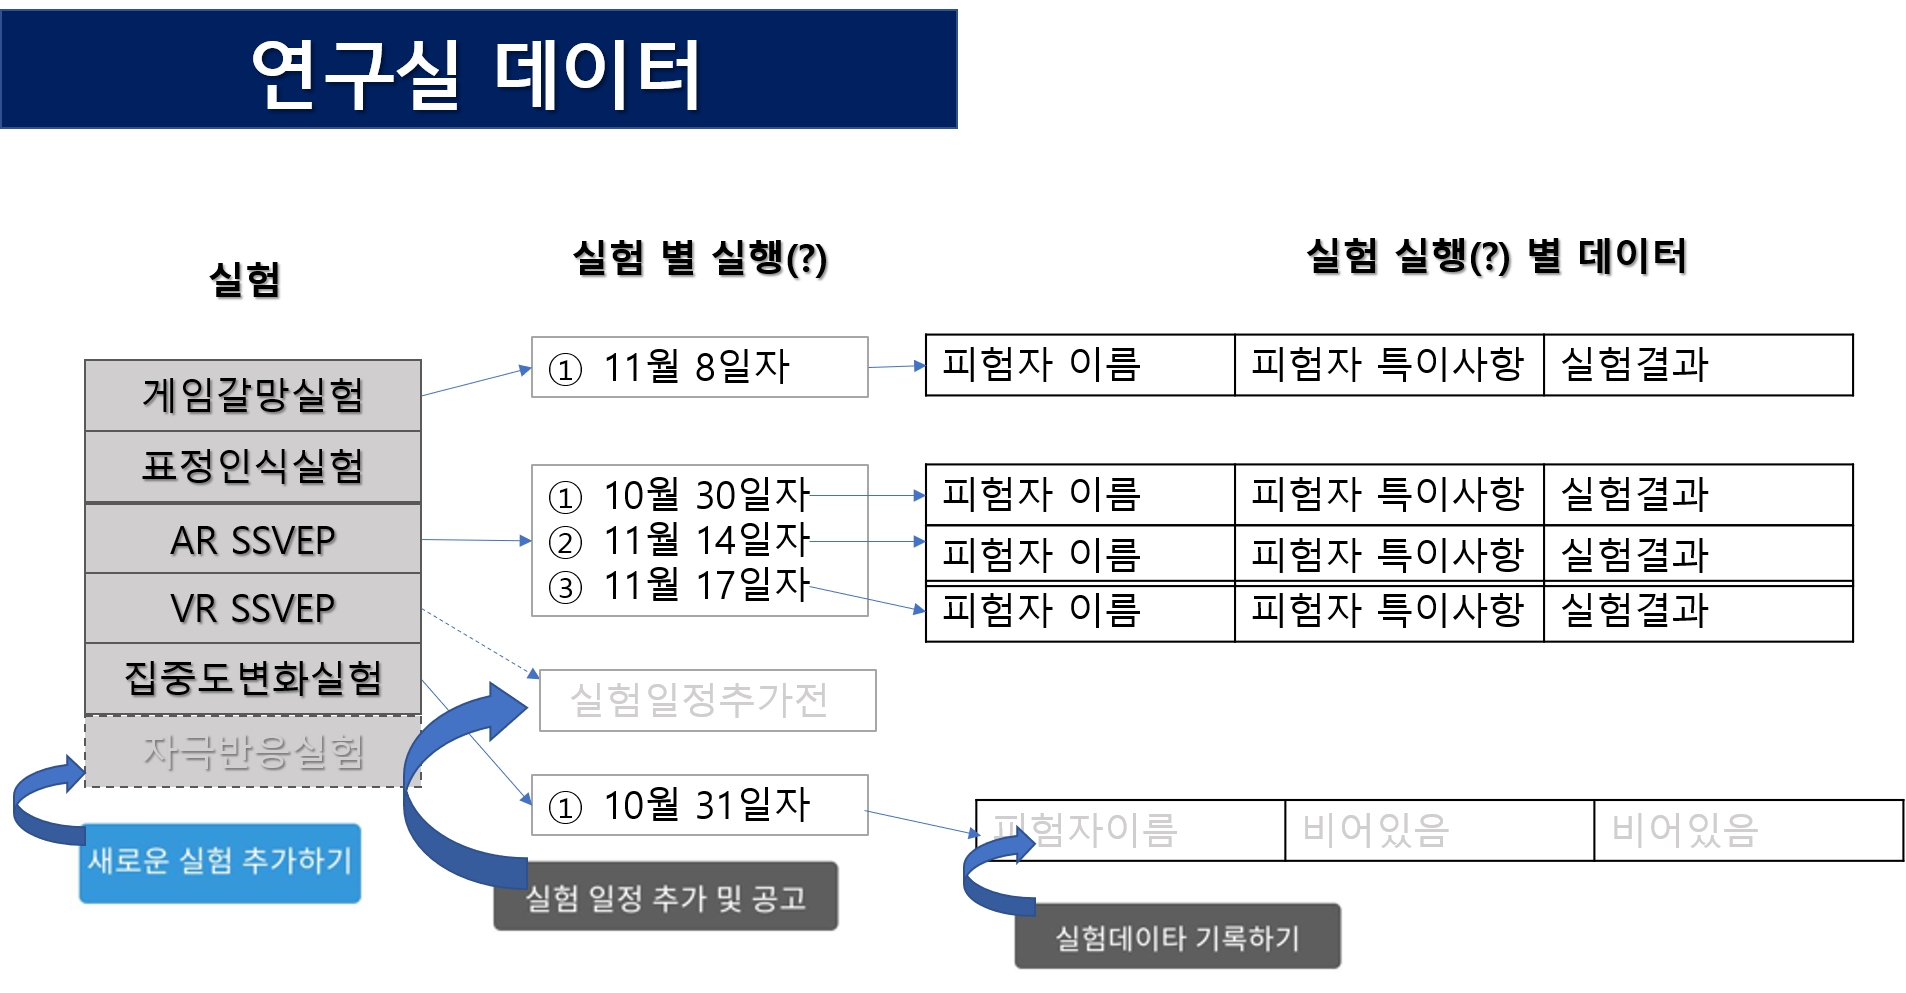
\includegraphics[width=0.5\textwidth,height = 7cm]{Oven/14_structureOfExperimentData.png}
The above image shows the structure of database. For each experiment instance (Experiment Model), several conducting schedules (Experiment\_Details Model)  is connected. Then for each of the conducting schedule, experiment result data(Experiment\_Result Model) are connected. \\


\subsubsection{CreateExperimentTable.php}
The leftmost button in the image indicates registering an experiment project. Researchers input information according to table. The notice goes up according to the  form. It  contains  id, name, poa, background, tester-name and time stamps.\\
\subsubsection{CreateExperimentDetailsTable.php}
The button in the middle indicates registering new schedule for the experiment to be conducted. The notice goes up according to the  form.  It  contains  id,  experiment-id,  name,  poa,  background,  tester-name,  objective,  location,  time-taken,  payment, method-desc,  end-recruit-date,  required-applicant,  applicant,  date- time and time stamps. In this, 'experiment-id' column refer to id of Experiment Table. This allows it to know what kind of project this small experiment is about. Researchers input information according to table.\\
\subsubsection{CreateExperimentResultTable.php}
The rightmost button indicates registering results of the experiment that has finished conducting. Researchers input information  according  to  table.  Researcher’s  experiment  results are saved in table. It contains ID, experiment-id, participant-id, file, remark, time stamps and date-time. In this, 'experiment-id' column refer to id of Experiment-Details Table.\\
\subsubsection{CreateParticipantsTable.php}
Register information of participants . Participants  input  information according  to  table.  It  contains  id,  experiment-id,  exp-name, user-id, name,  status,  date-time and time stamps. In this, 'experiment-id' column refer to id of Experiment-Details Table.\\
\subsubsection{UserMyPageController.php}
Check the currently logged in user with auth:user() to import Participants instance that has ‘user-id’ of that user. comparing experiment-id of participants instance with id, import and list the experimental-Details of user. User can cancel their applying. In cancelling, it send the id of the Experimental-Details instance in the list to parameter. If this parameter value is the same as the ‘experimental-id’ and id 0f currently logged in user is same as ‘user-id, delete it. Then, the applicant column value of the Experimental-Details instance that has same id with ‘experiment-id’ is reduced by 1\\
\subsubsection{ResultRequest.php}
It contains rules, message and attributes function that need to be applied when the admin sends a request to store the experiment result data into the table.  Rules contains  file, remark, experiment-id, participant-id, date time and status. ‘file’ contains information about the physical path where the uploaded file is located and it requires the size of file being uploaded to be under 20MB. ‘remark’ means comment which the special attention is need for the subject and it is required, ‘experiment-id’, ‘participant-id’ and ‘date-time’ are also required.\\
\subsubsection{UserHomeController.php} 
Participants fill out the form. It contains id, experiment-id, experiment-name, participant-name, status, date-time. Participants information will be saved according to the form. Obtain the candidate object from the user table and the experiment table of the DB. The number of applicants for the notice increased by 1. It is not implemented if it has already been applied or if it has been recruited.\\
\subsubsection{ExperimentResultController.php}
Save the experiment-result file. Check if a folder with that name  exists,  and  if  it does not exist, create the folder with make directory method of ‘file'.\\
\subsubsection{RedirectIfAuthenticated.php}
Decide  where  to  redirect when you are Authenticated.\\

\maketitle{\textbf{construct()\\}}
The functions in the Controller are available only when current user is admin.\\ 
\maketitle{\textbf{create()\\}}
Bring   up   a page  to  save  the  experiment  results.  Using  id  value  get  by Request,  hand  over  the  subject’s  data  corresponding  to  the experiment  results.  It  passes  on  information  on  which  of the Experimental-Detail Models you have experimented. And when the Create Results page is returned, the data is handed over  together. \\
\maketitle{\textbf{show()\\}}
Upload  the  page  where  the  subject’s experiment results are stored. Check the subject model with the  parameter  id  value.  Hand  over  the  User  information corresponding to the Participant. The results of the same kind of experiment that the subjects participated are inquired with the parameter id.\\
\maketitle{\textbf{store()\\}}
Store  the  Experiment  data  of  the  subject.  Store  the information  received  in  the  Post  method  per  column  in  the new  Experimental  Result  Object.  The  status  of  the  subject changes  from  To  be  Determined  (TBD)  to Completed Work (CW) when the experiment results for that subject are saved. Save the  test  result  file  if  it  exists.  Check  if  a  folder  with  that name  exists  within  the  Public  folder,  and  if  not,  create  the folder with Make Directory method of File. It save  public  file  route  in  column and configure the file name as subject name, experiment name, experiment number  to  save  with  the  file  type.  Store  the  address  of  the actual path in the file column, Used to refer to a file in the physical path.\\
\maketitle{\textbf{delete()\\}}
Delete the experiment results whose status column is CW from the subject’s table. Store and inquire the subject id of the experiment result to be deleted. It only deletes the contents  of  the  table.  So,  after  receiving  the  address  of  the”file” column of the table, use the delete method of the file to  go  to  the  actual  address  of  the  file  and  delete  the  file.Among  the  experimental-result  data,  the  subject  id  column finds  a  model  that  is  equal  to  the  value  of  i  and  erases  the data  from  the  table.  When  all  deletion  is  complete,  return response.\\
\maketitle{\textbf{delete-user()\\}}
Used  to  delete  a  candidate  from  the  list  of candidates to be tested. Check the applicant who applied for the  test  notice  with  the  parameter  id.  Delete  the  candidate corresponding to the id value from the Participant table. The number  of  applying  persons  in  the  application  column  in the  test  announcement  table  is  reduced  by  1  because  the applicants for the experiment were deleted. When all deletion is  complete,  return  response.\\
\maketitle{\textbf{download()\\}}
Download  the experiment result file. Grant permission to access to account‘admin’.  Check  the  experimental-result  data  corresponding to the id. The actual file path value saved in the file column of the retrieved data is given. Return response by putting a file path value in the Download() method.\\





\subsection{Display Design} %동수 워드파일 반영된 곳
\subsubsection{style.css}
It is a self-produced css file. I configured the style by adding a class that does not exist in the bootstrap or template oneui.css. We have also added a number of classes for responsive webs using media query.\\
\subsubsection{fullcalendar.css}
A calendar design file that is essential for experiment scheduling. And this file is used with fullcalendar.js file.\\
\subsubsection{fullcalendar.js}
A js file that contains basic information about calendar behavior. Refer to the classes in fullcalendar.css here to record the behavior for the button.\\
\subsubsection{bootstrap.min.css}
A bootstrap design that consists of a class of optimized styles for reactive types.\\
\subsubsection{oneui.css}
It is a bootstrap based template and has many classes. I can import and use classes that are essential for project front-end configuration.\\
\subsubsection{lang-all.js}
Basically, it provides a function to modify the English language set in the fullcalendar.js file to suit the language of each country. I created a Korean calendar by referring to lang-all.js and specifying 'ko' as the default language in the jquery script file that specifies the calendar value.\\
\subsubsection{app.js}
It contains the main functions for using the header function. We set up user interface init, declare uiInit as a variable, and use jquery to create the behavior for the main functions used in the header. In particular, I created a function that declares the header-navar-fixed class so that the header size is fixed even if the scroll size is exceeded.\\
\subsubsection{show.blade.php}
This php file is a page where users can select the experiment they want and apply for information such as eligibility, time and salary. We have added a property to the calendar that indicates whether the recruitment is over or not, so that we can apply for a more efficient experiment. I created a jquery function and referenced the fullCalendar class with  ('calendar'). fullCalendar in it. In the event attribute, variables were set so that the experiment name, completion of the recruitment, experiment researcher name, and experiment time can be displayed for each calendar date. Since I could not output up to four basic attributes, we declared eventRender as follows.\\
\maketitle{\textbf{eventRender()\\}}
element.find('.fc-title').append("<br/>" + event.time);\\
element.find('.fc-title').append("<br/>" + event.tester); \\
element.find('.fc-title').append("<br/>" + event.condition);\\
\maketitle{\textbf{events:[]}}
we bring the value(columns) in database from  app/Http/Controllers. So, I added the value of the fullcalendar attribute to the scripts. A total of four display values were retrieved from the DB and displayed on the calendar.\\
\subsubsection{header.blade.php}
The header.blade.php file contains basic attribute values that are imported from all the front php files. I have referenced all the css files, fonts, images, js files etc that I need to refer to, and I have added the homepage icon, KakaoTalk preview image, and a brief description of the homepage using the meta property. I also added my own script file. The code shown below is the logic of the page header portion, which is common to all pages. I used jquery to code the header, login, and my page menu to be included in the button when the size of the mobile device became smaller. When you click the button, the menu will drop down in the drop-down format as if it were created in the header bg class, and the rest of the screen will be displayed in black.
In addition, I created the arrow list class and designed the logic to return to its original state by clicking the arrow.\\
\subsubsection{index.blade.php}
This file under the mypage directory is the My Page of the user who wants to experiment. Through this page, you can check the lists you have applied, and you have unintentionally implemented a function that allows you to select and delete experiments. The table header function selects all the checkboxes in the table when you click the checkbox in ‘thead’.\\







\subsection{Account Management}


\maketitle{\textit{\\Page01:Choosing User Type\\}}


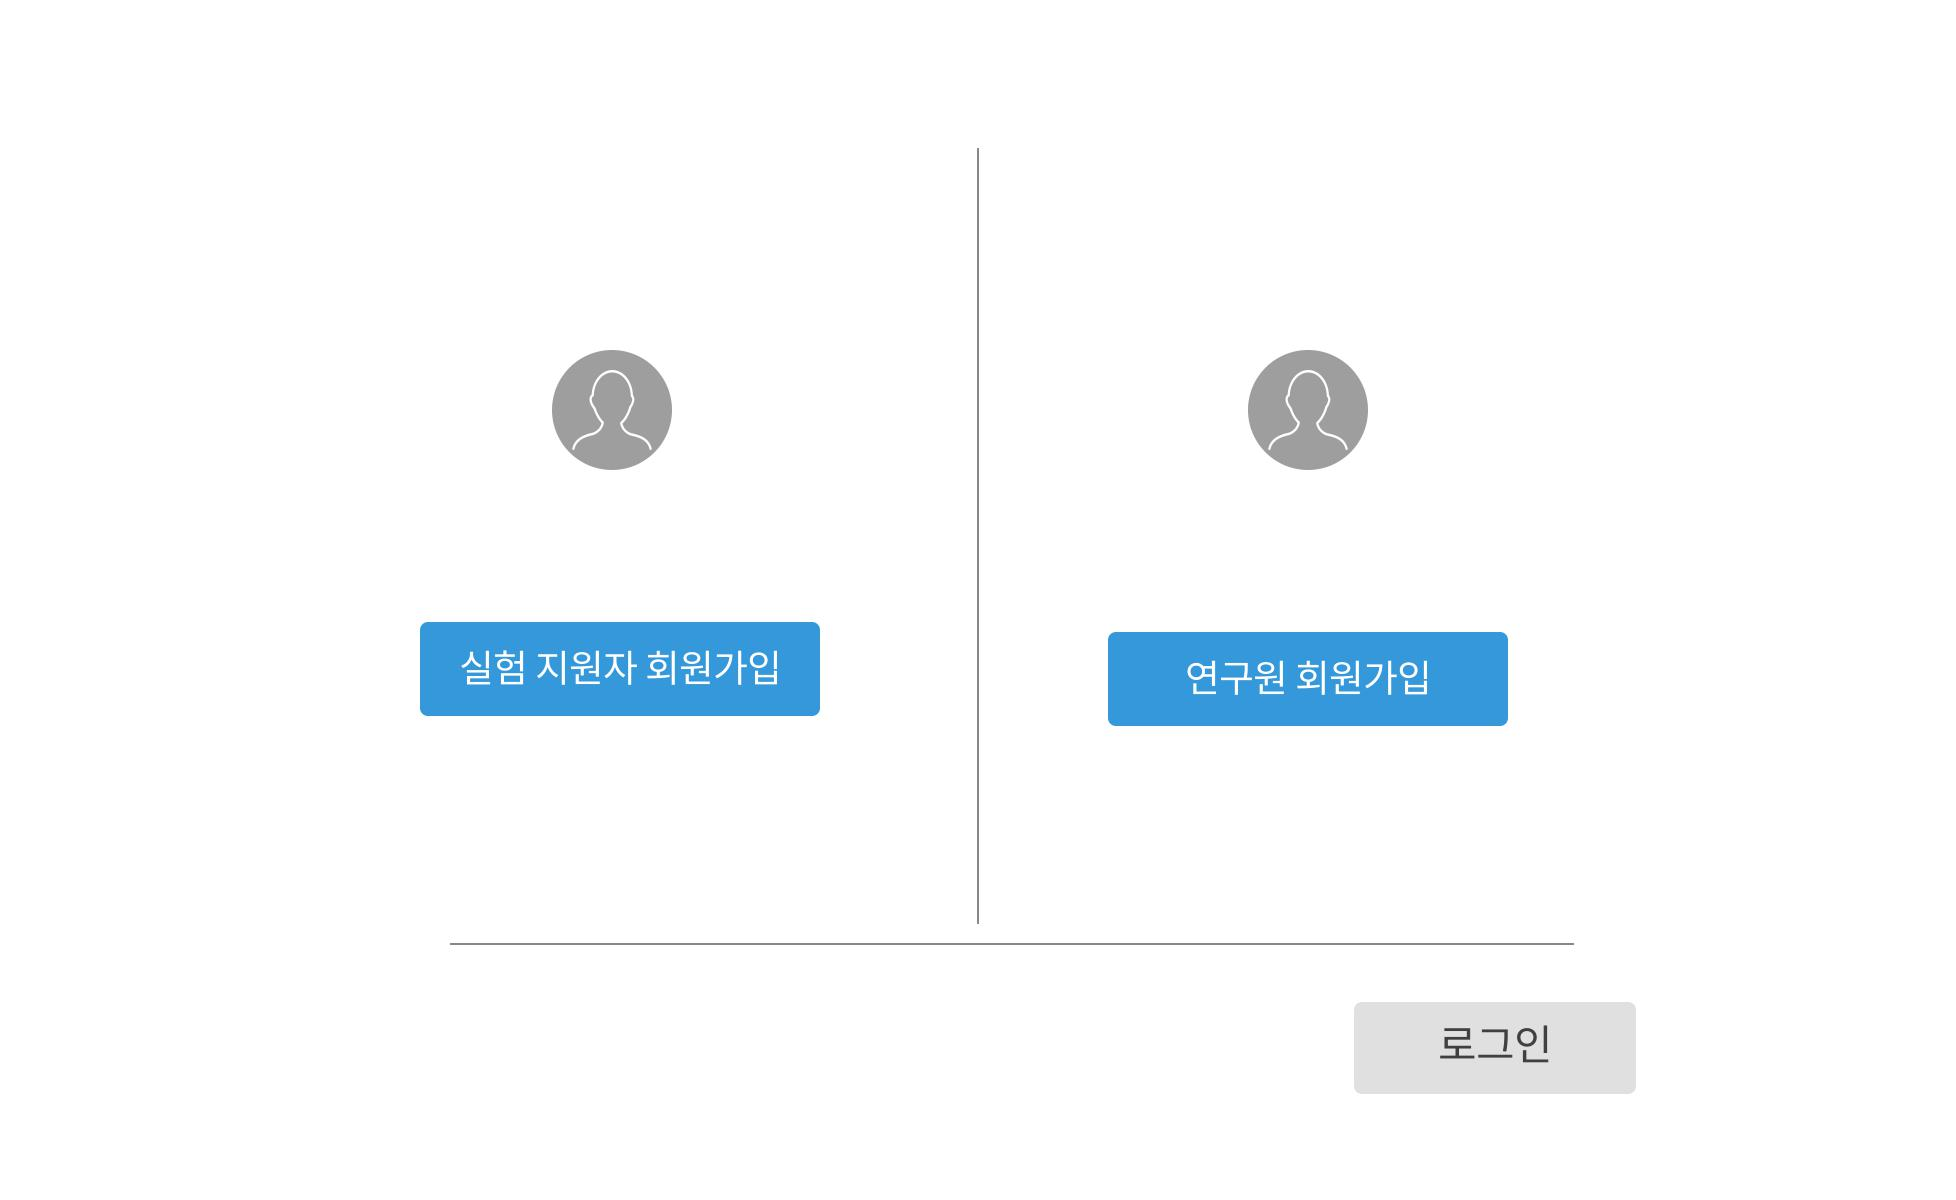
\includegraphics[width=10cm,height=8cm]{Oven/01_firstpage}

\subsubsection{Separate Account Data}
At the very first page, users should check whether they are lab researcher or applicant. After choosing their type, then the sign up and sign in page will be shown like above. The information of users should be organized at MySQL database. Whether they registered as a lab researcher or applicants must be included in the column. The column which contains the type of the users will determine which of the two main pages will be selected at the server. \\

%%%%%%%%%%Table of Underlying Class Or Function%%%%%%%%%%%%%%%%%%%%
\begin{supertabular}{ |p{3cm}|p{4cm}| }
 \hline
 \multicolumn{2}{|c|}{Underlying Class Or Function} \\
 \hline
 HomeController.php & Separately manage researcher's account and applicant' account. Show home page that contains routes to user sign-in/ sign-up and admin sign-in/ sign-up.\\
 \hline
\end{supertabular}
%%%%%%%%%%%%%%%%%%%%%%%%%%%%%%%%%%%%%%%%%%%%%%%%%%%%%%%%%%%%%%%%%%%%%%%

\subsubsection{Sign Up}
Applicants and researchers can register with email address and password. 
If users click the register below, the message saying that the sign up process is successfully done will be shown. In that page, users can click the log in button which will pop the sign-in pop up window.

\maketitle{\textit{\\Page02:Sign Up For Researchers\\}}
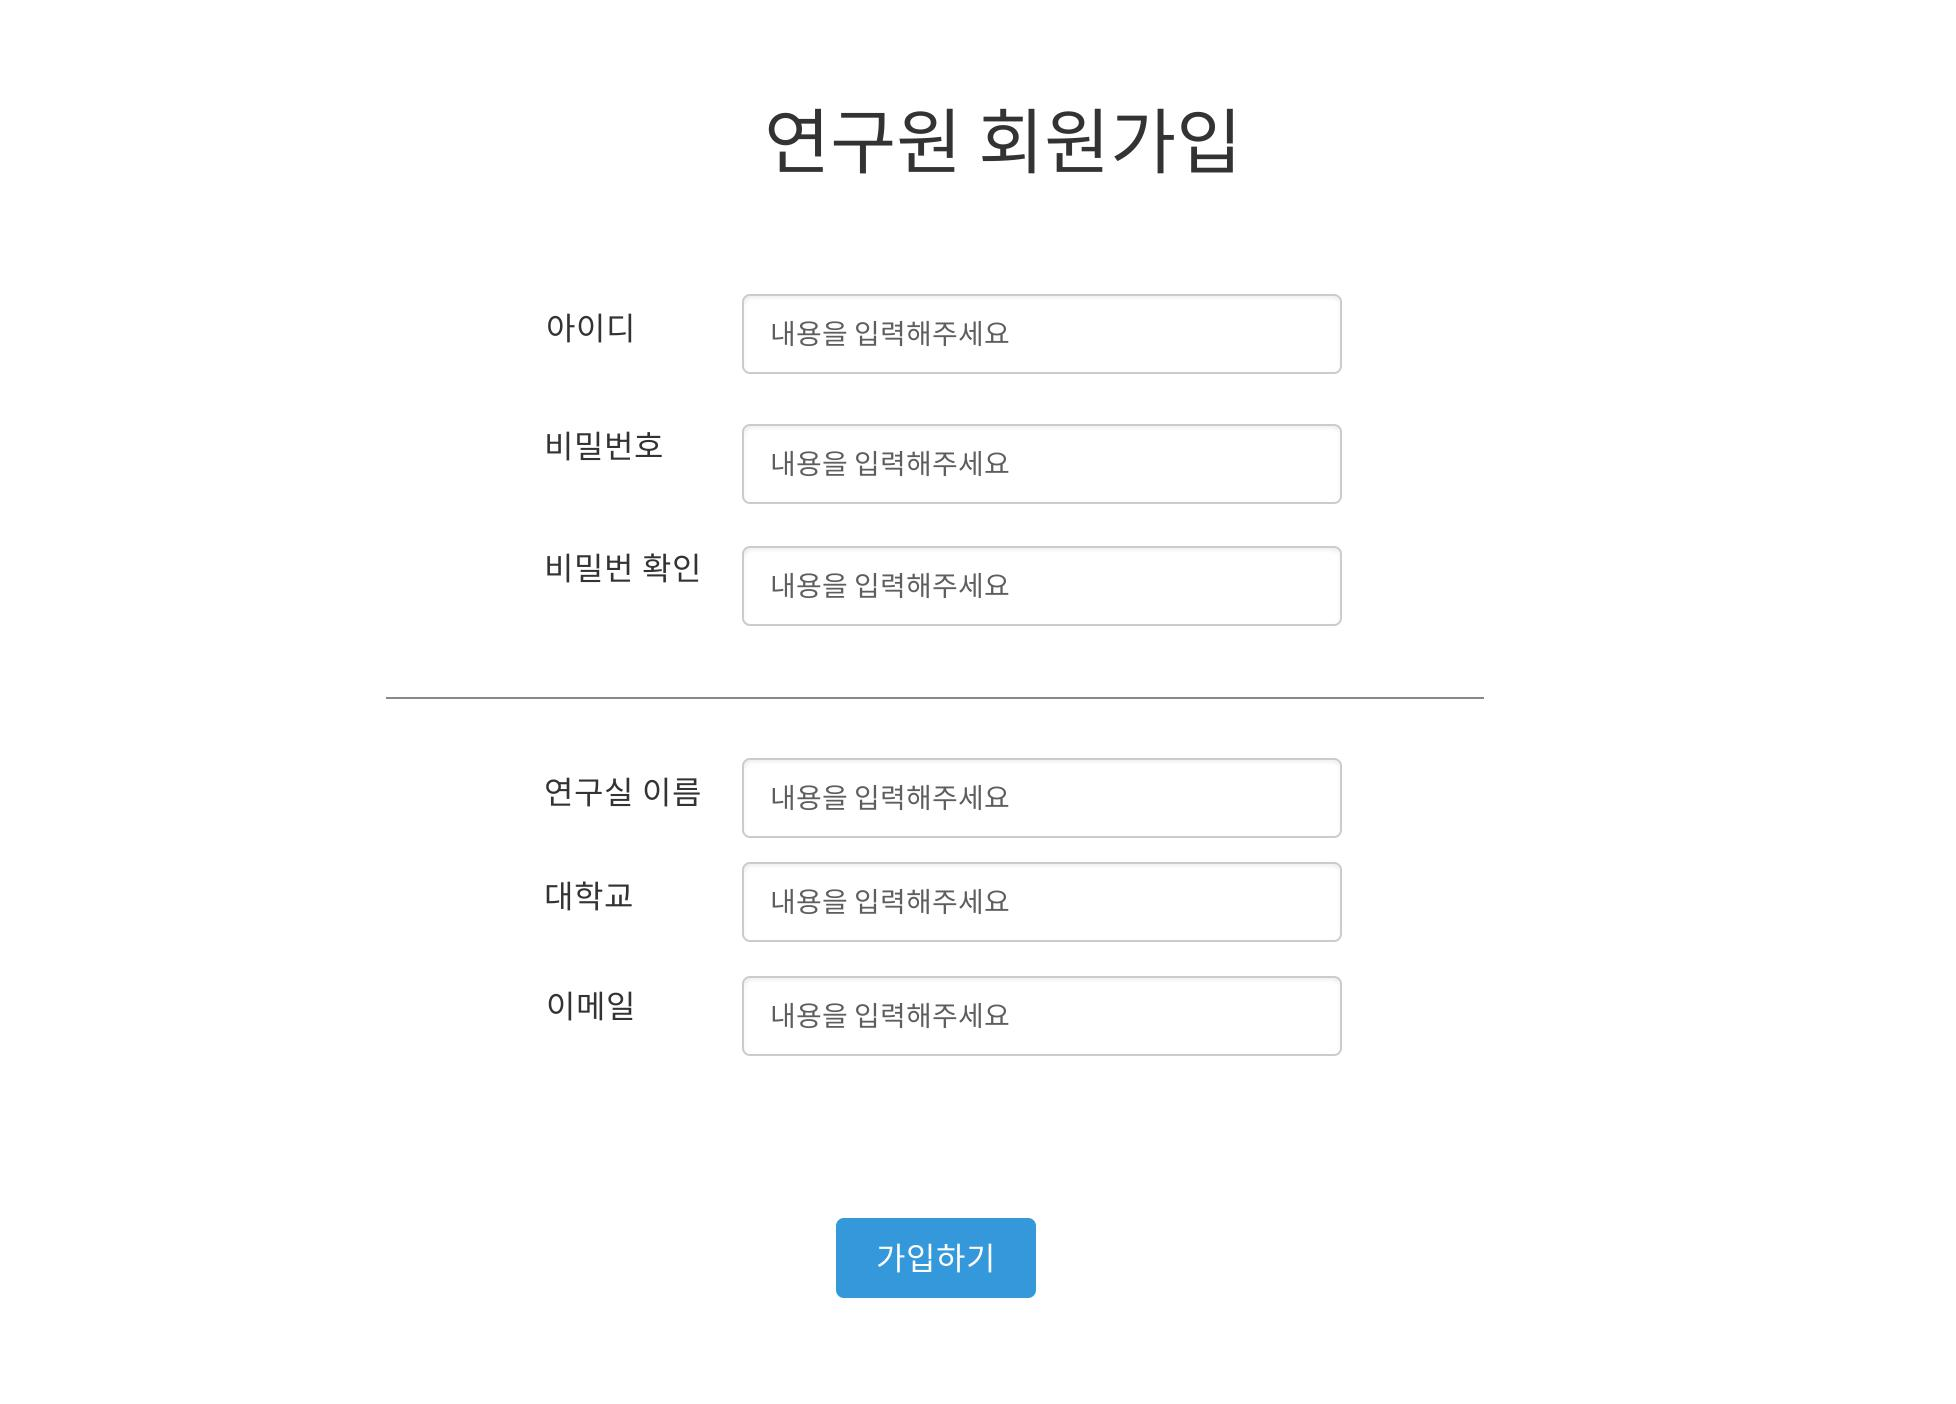
\includegraphics[width=10cm,height=8cm]{Oven/04_labSignup.jpg}
\maketitle{\textit{\\Page03:Sign Up For Applicants\\}}
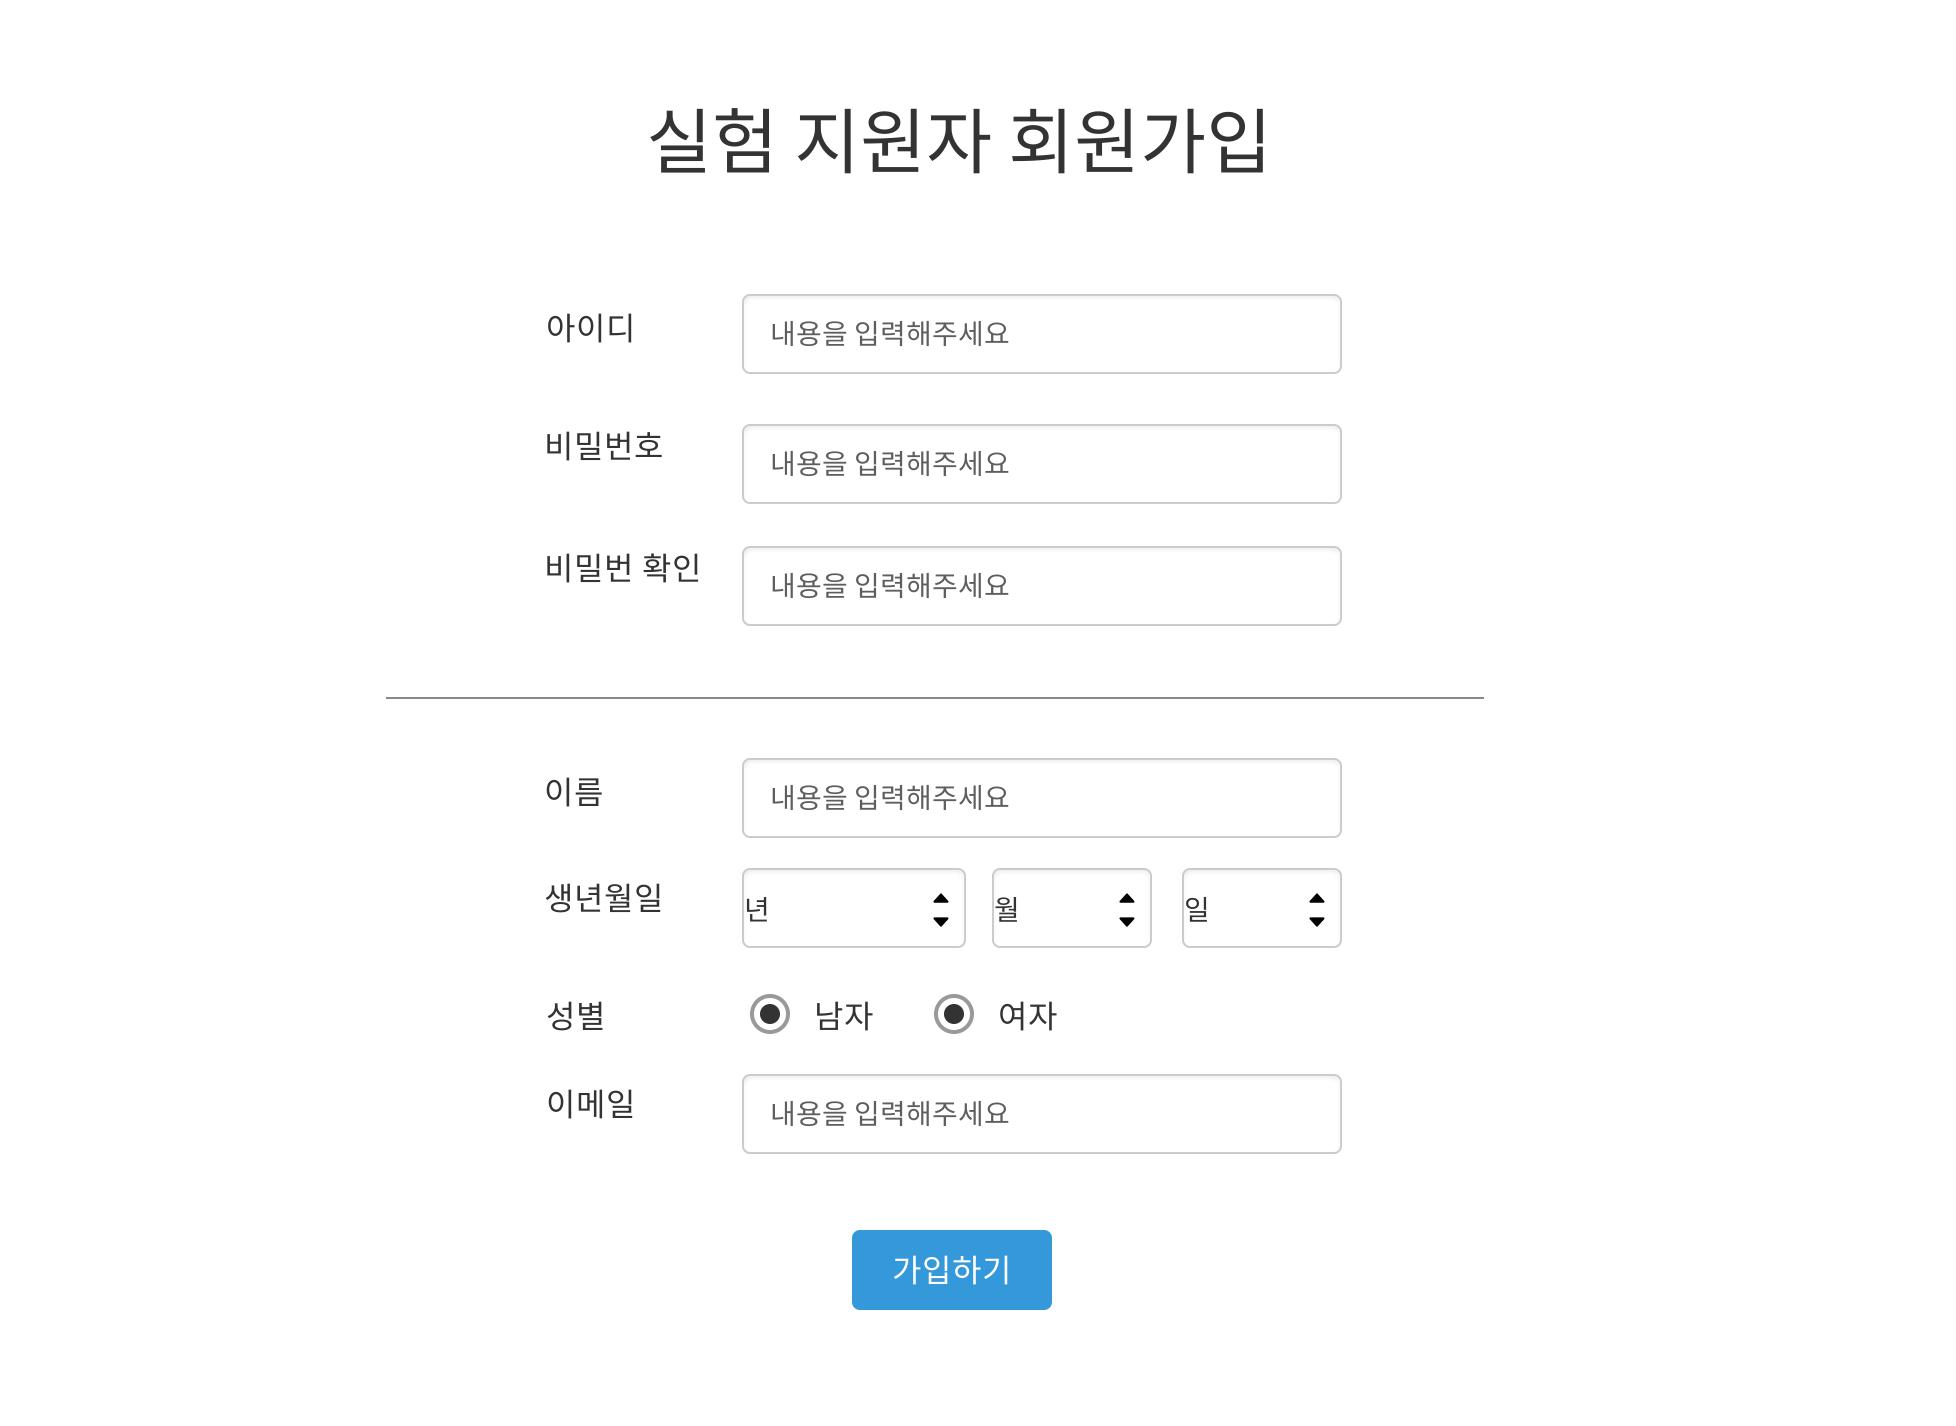
\includegraphics[width=10cm,height = 8cm]{Oven/03_applicantSignup.jpg}
\maketitle{\textit{\\Page04:Sign Up Completion Message\\}}

\includegraphics[width=10cm,height = 5cm]{Oven/05_signupCompleted.jpg}



\subsubsection{Log in}
Users can select whether they are applicant or researcher. Then they have to enter ID and PW correctly. Then click the log in button. According to user's member type, different main page for lab researcher or applicants will be shown.\\
\maketitle{\textit{\\Page05:Sign In\\}}
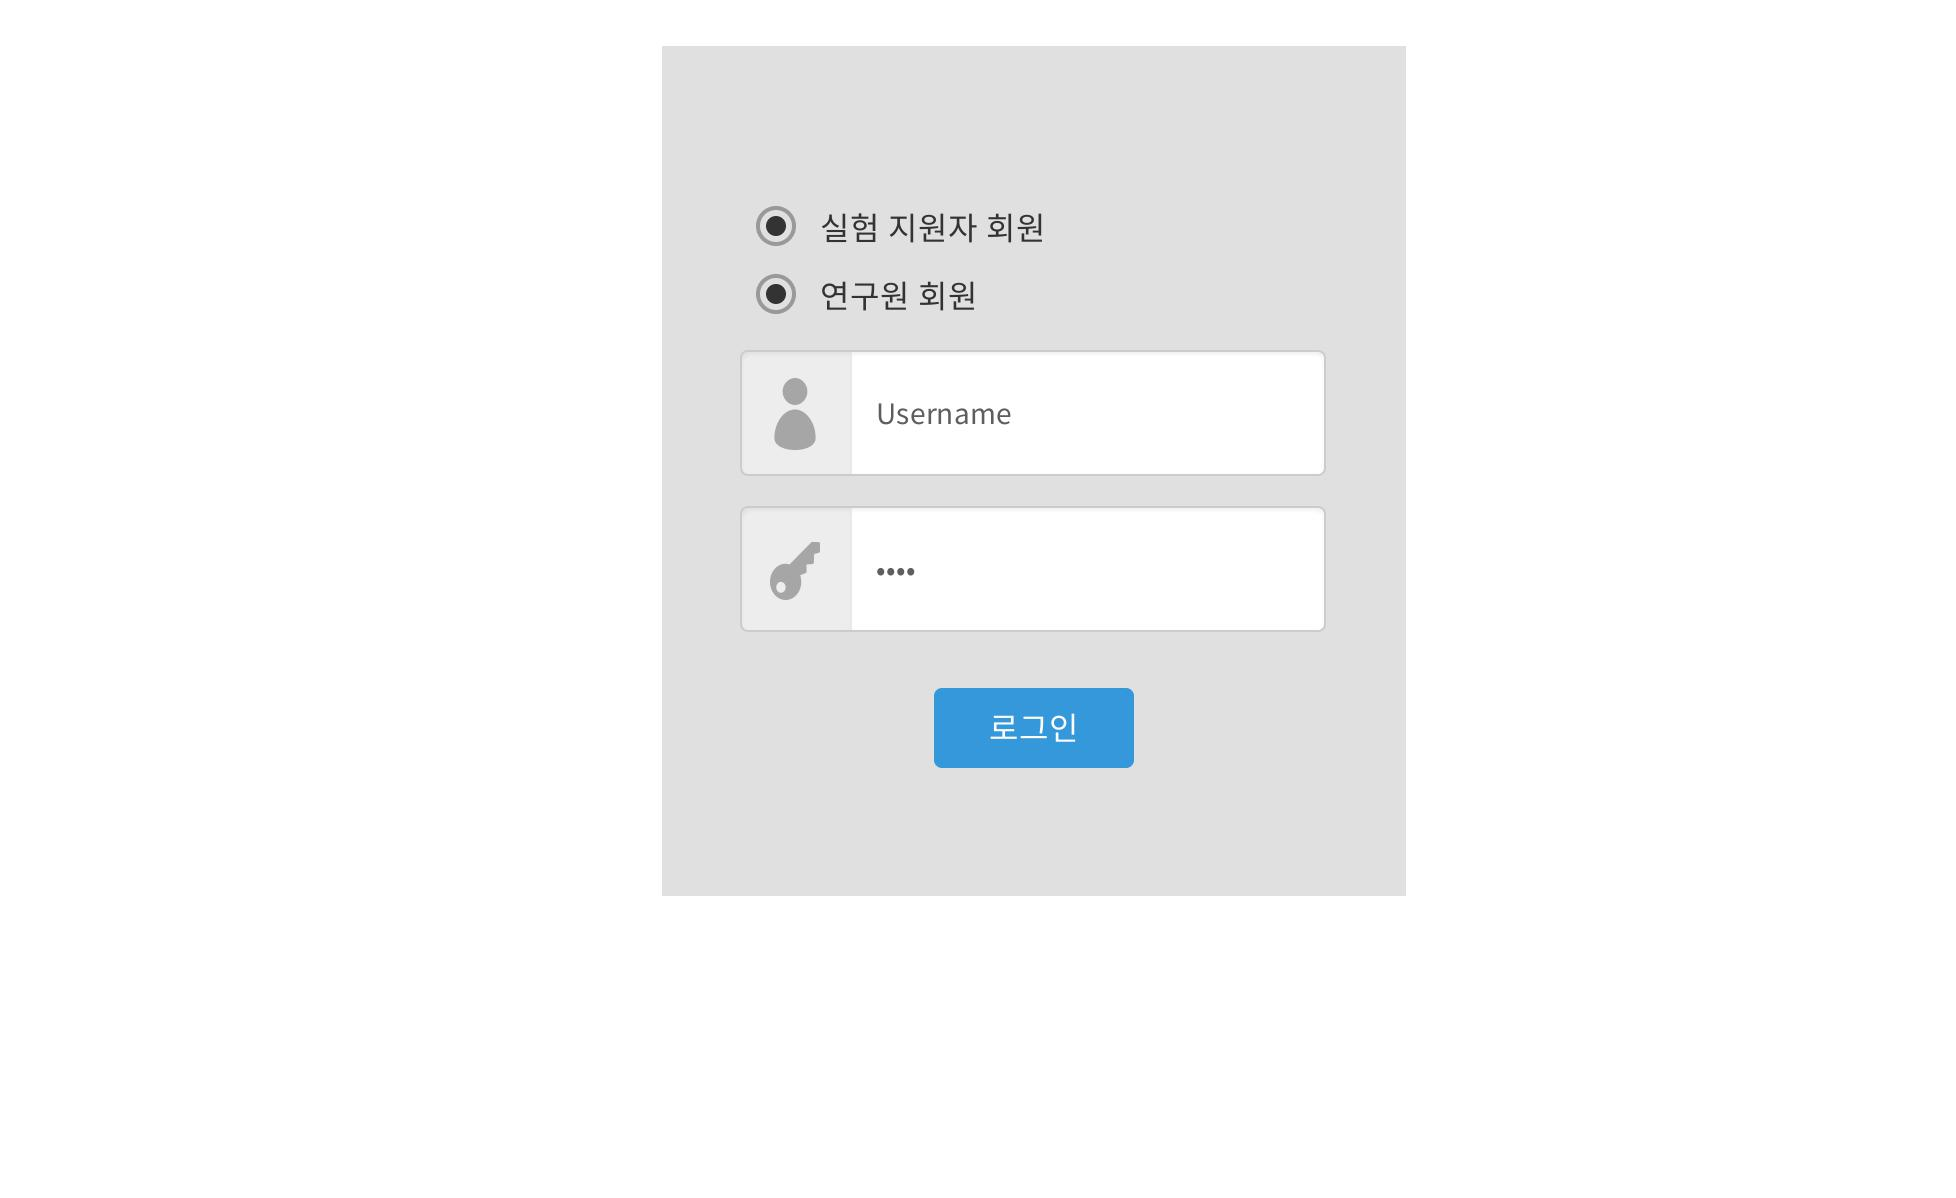
\includegraphics[width=10cm,height = 8cm]{Oven/02_signin}


\subsection{Functions For Lab}
\subsubsection{Main Page\\}
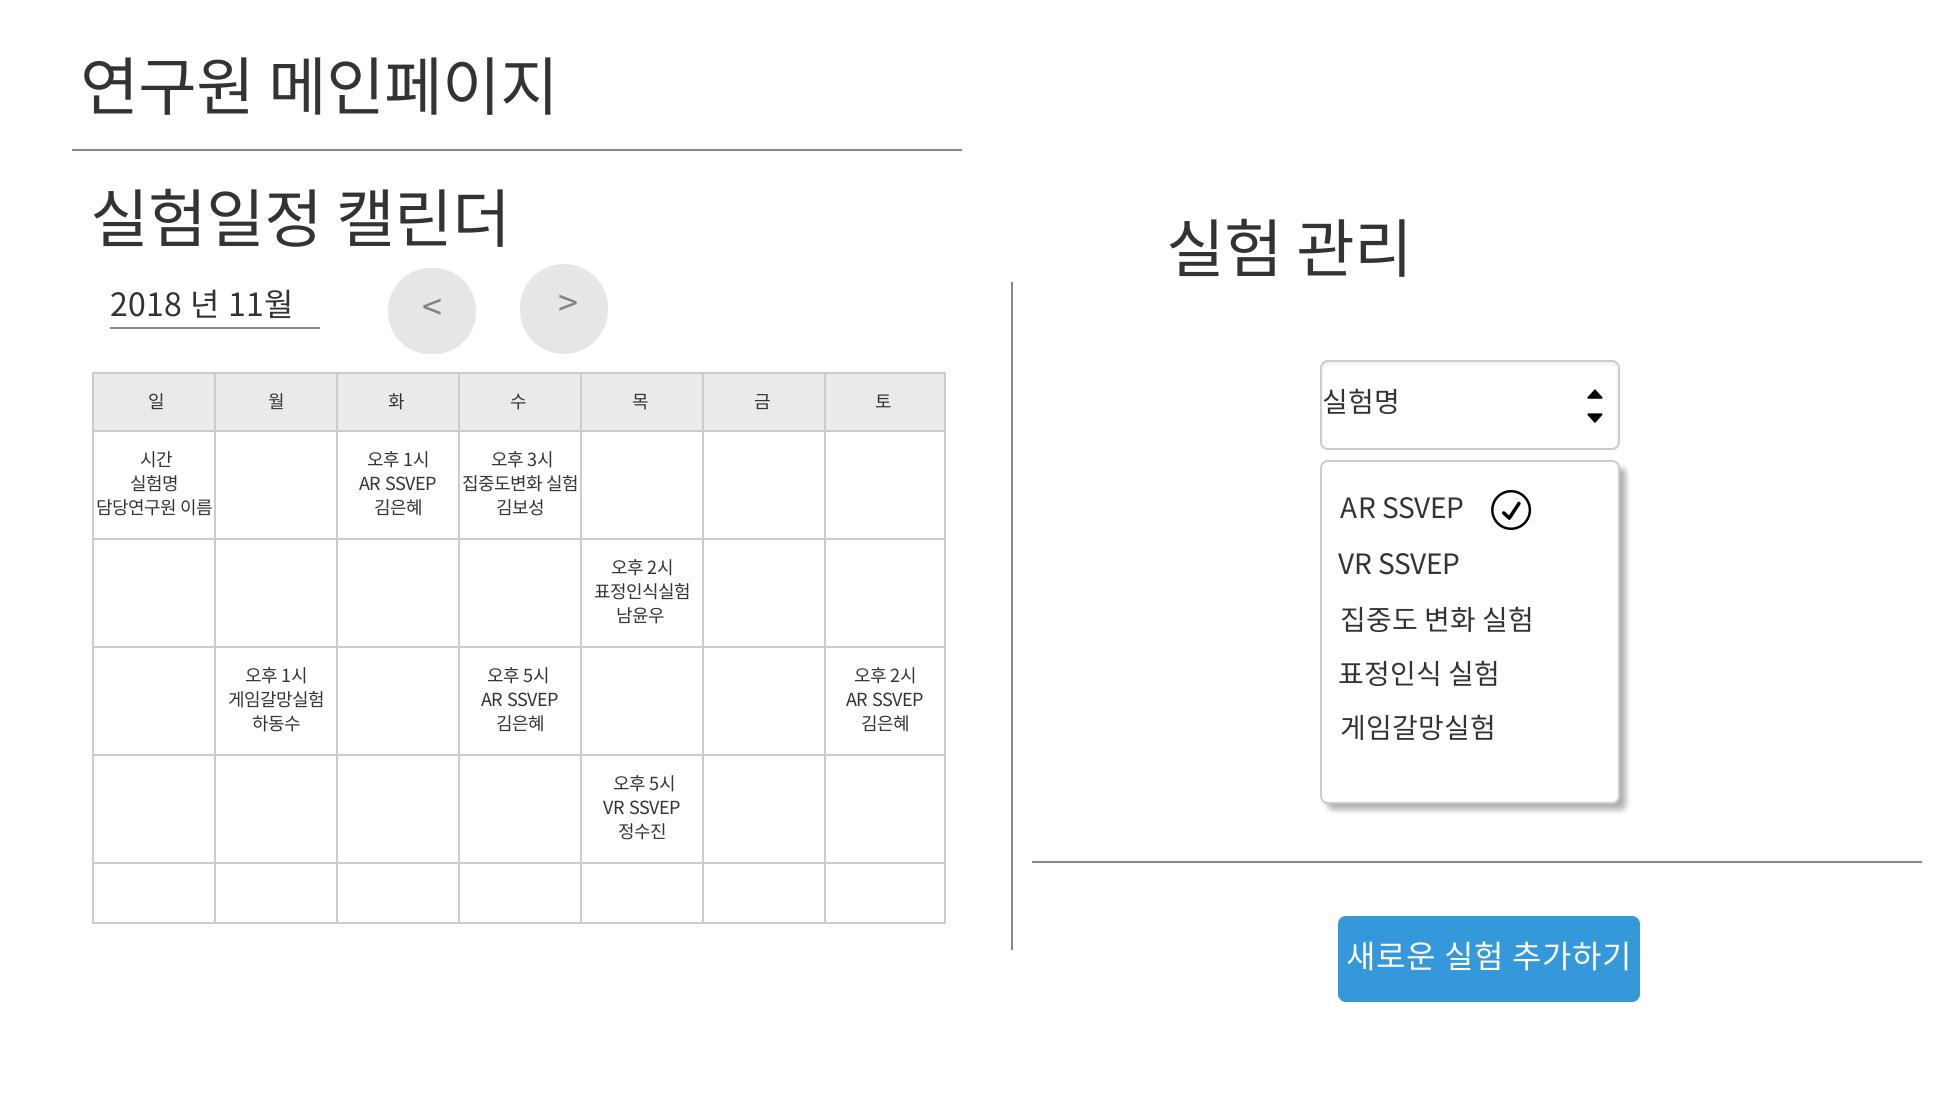
\includegraphics[width=10cm,height = 7cm]{Oven_ver2/ver2]06_labMainPage.jpg}

\begin{itemize}
\item Experiment Schedule Calender : Similar as google calender. User can see all the scheduled experiments at the month at a glance. It also includes the experiment schedule that no applicants had applied. 
\item List of Experiment Instances With Drop Down List of Researchers In The Lab : This list will function as interface between main page and other functional pages. Just check one of the drop down elements and click the buttons below. 
\item Button For Creating New Experiment Instance
\end{itemize}

\subsubsection{Create Experiment Instance}

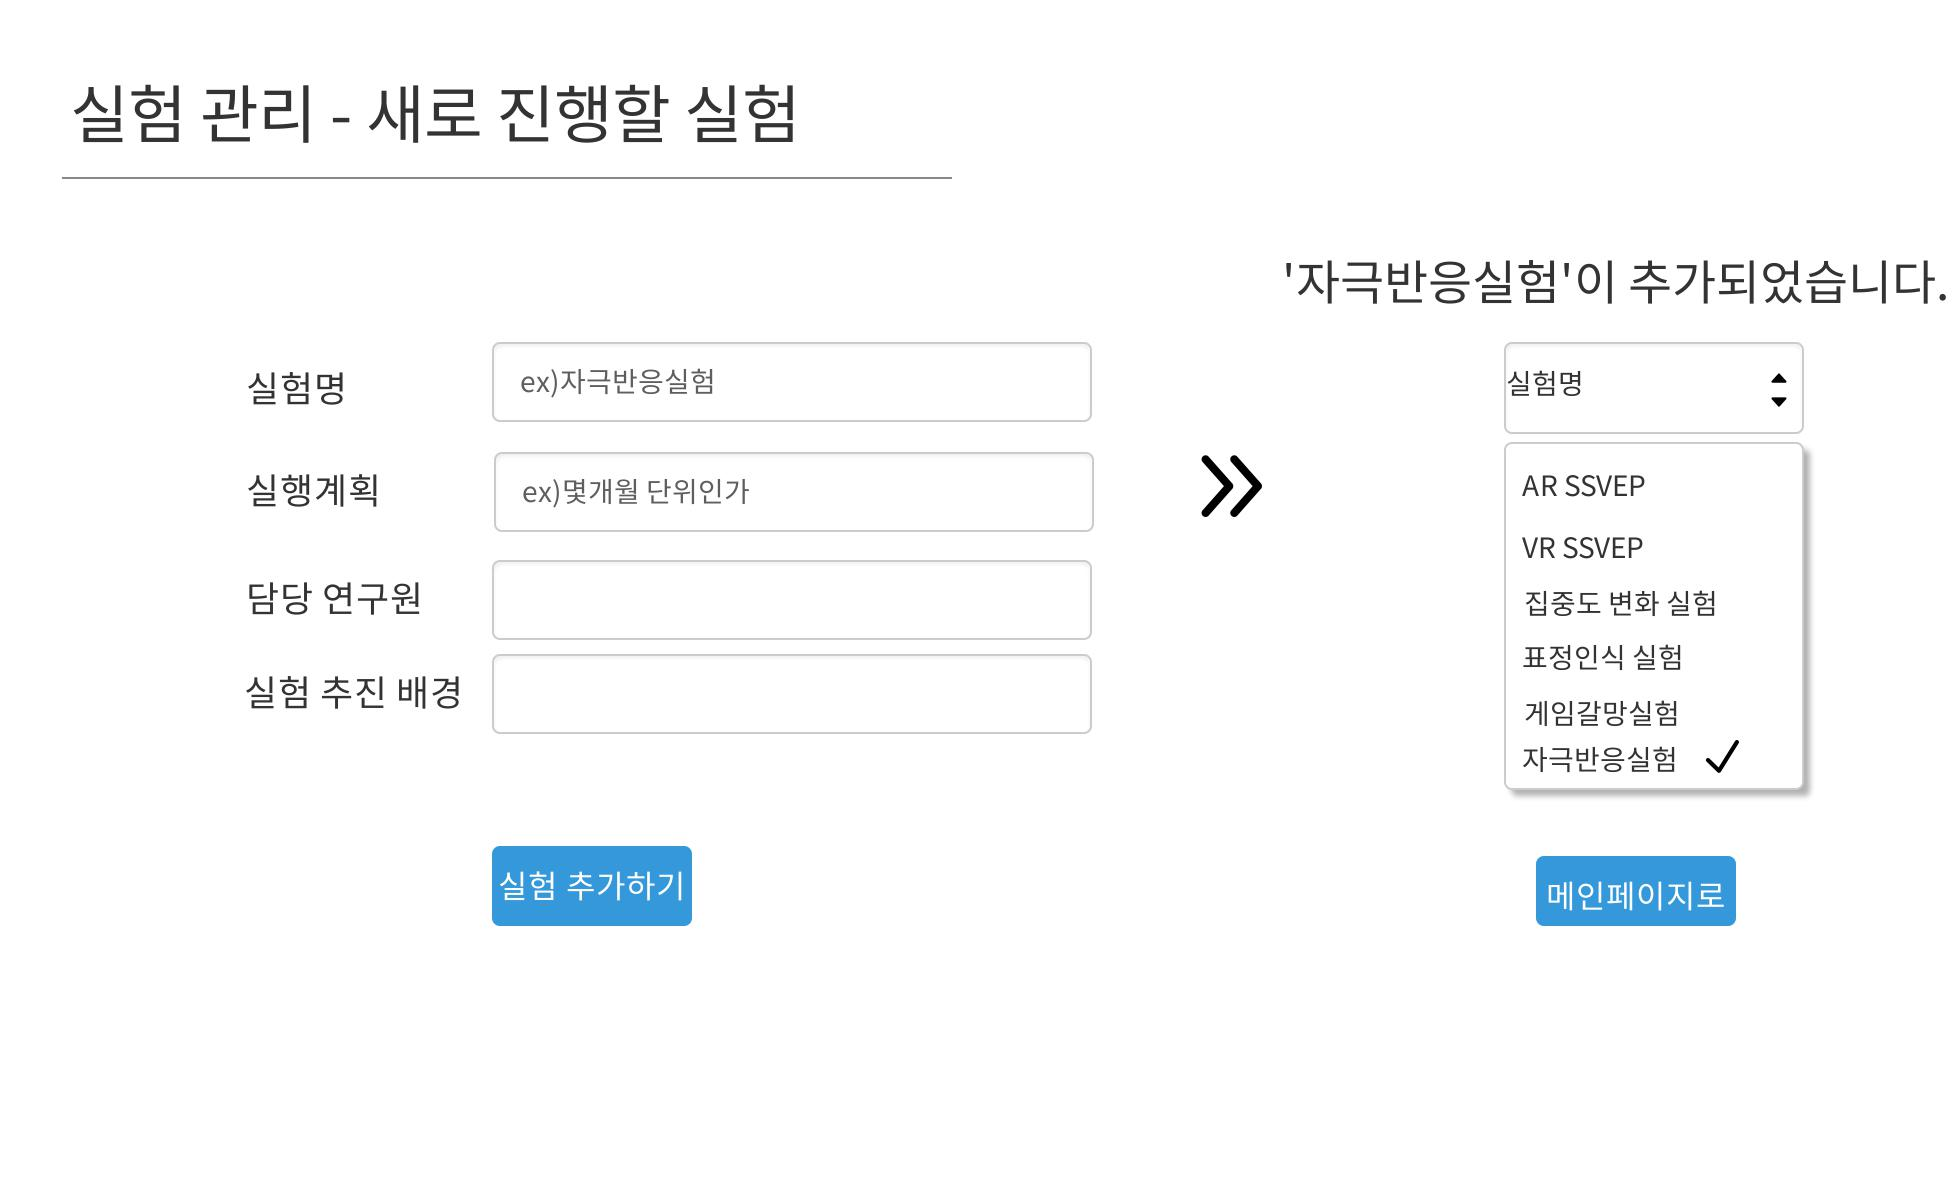
\includegraphics[width=0.5\textwidth,height = 7cm]{Oven/07_addNewExperiment.jpg}

When the lab researchers decided to hold a new type of experiment, the instance of that experiment should be created in database. Enter the name of experiment, expected schedule, researcher in charge and the purpose of it. \\


\subsubsection{Main Page For Experiment Instance\\}
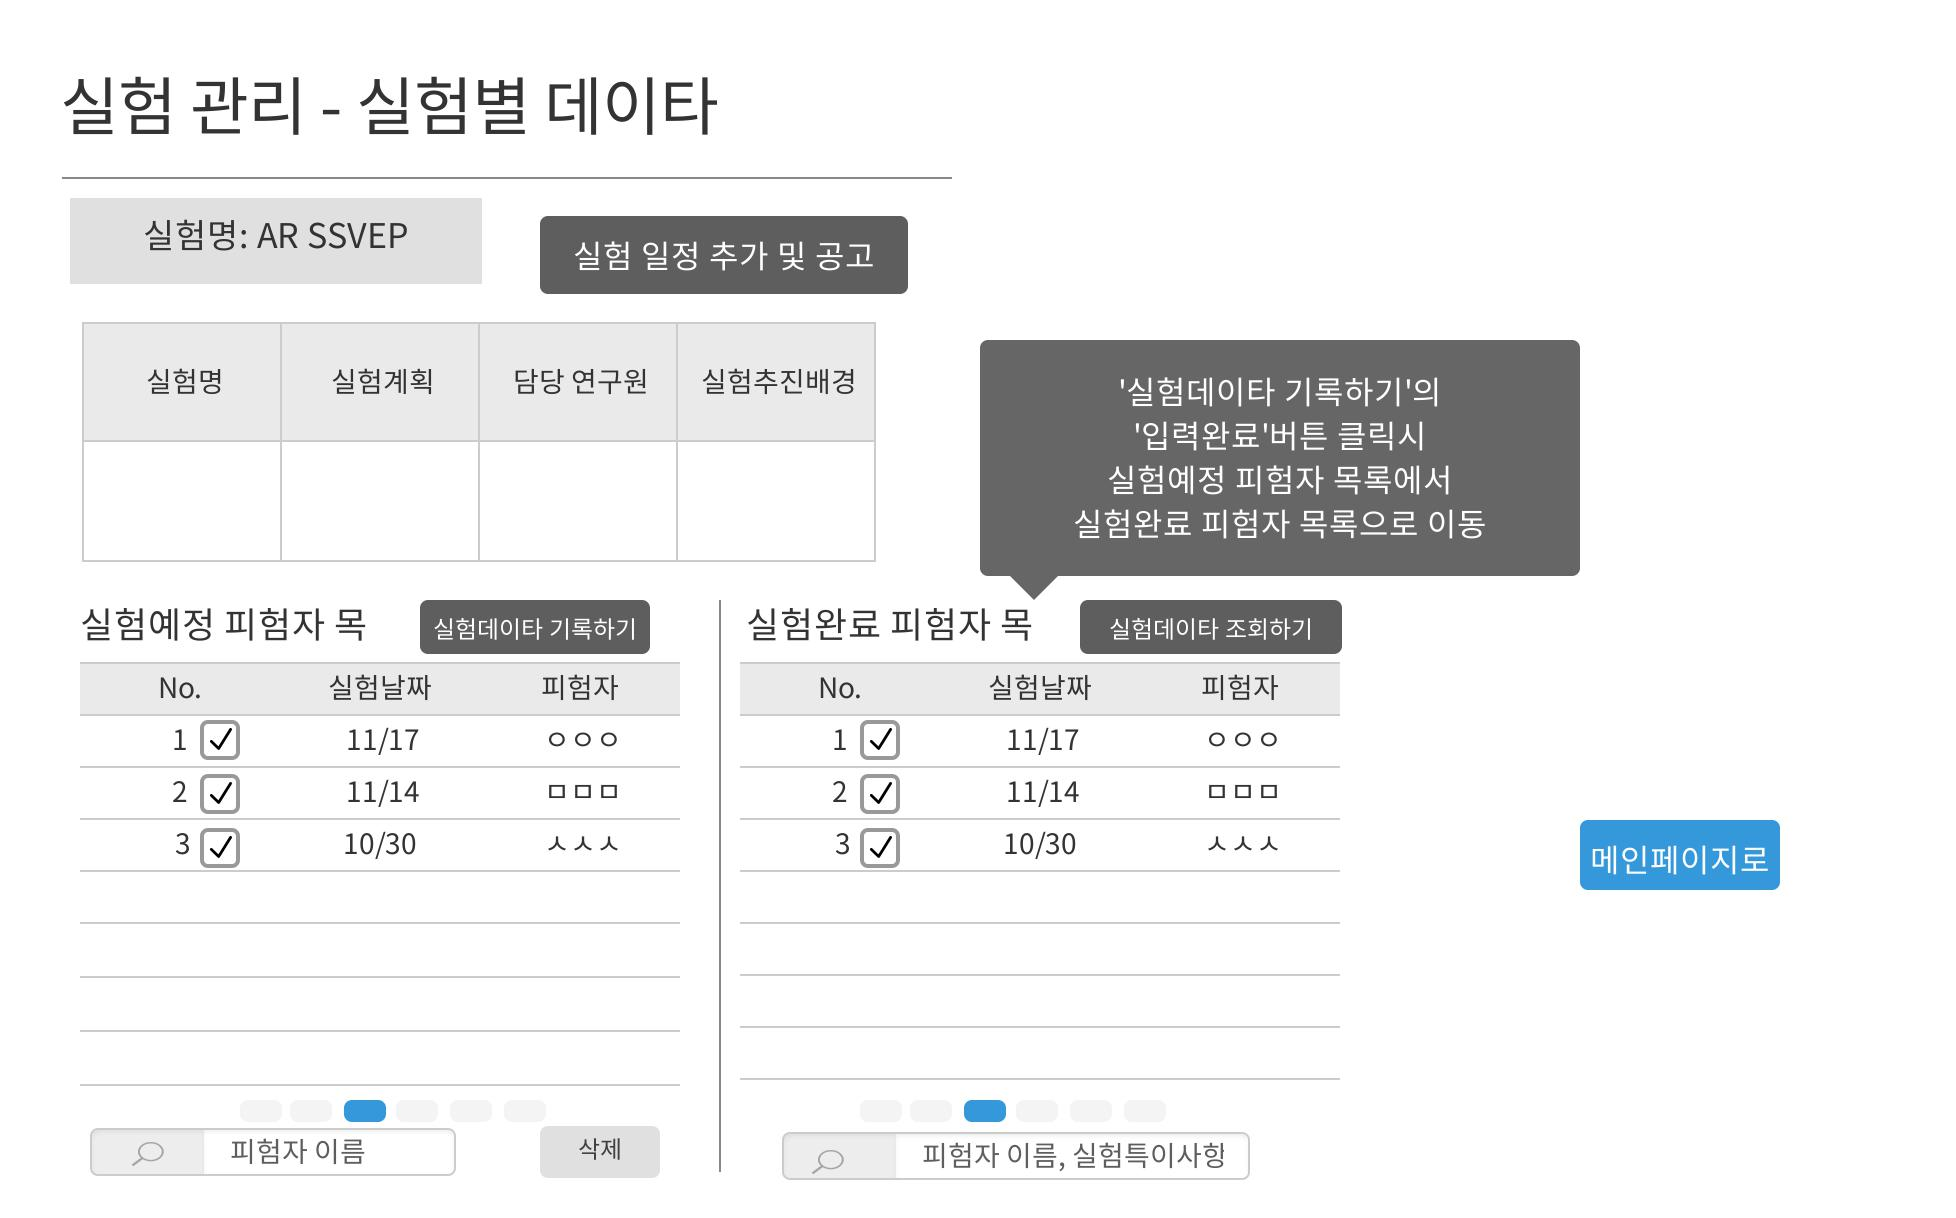
\includegraphics[width=10cm,height = 7cm]{Oven_ver2/18_subMainPage.jpg}
The most recently held experiments will be at the top of table. Lab researchers can search for a specific data by entering several information of applicants or key words about that experiment. 
\begin{itemize}
\item Information of experiment which is chosen at the drop down list.
\item Button For Posting Recruitment Notice 
\item List Of Applicants Who are scheduled but did not conduct yet.
\item List of applicants who have finished conducting experiment.
\item Search Bar For Applicant's Information
\item Button for cancel.
\item Button For Uploading Experiment Result Data
\item Button for reviewing uploaded experiment result data\\
\end{itemize}




\subsubsection{Reviewing Uploaded Experiment Result Data}
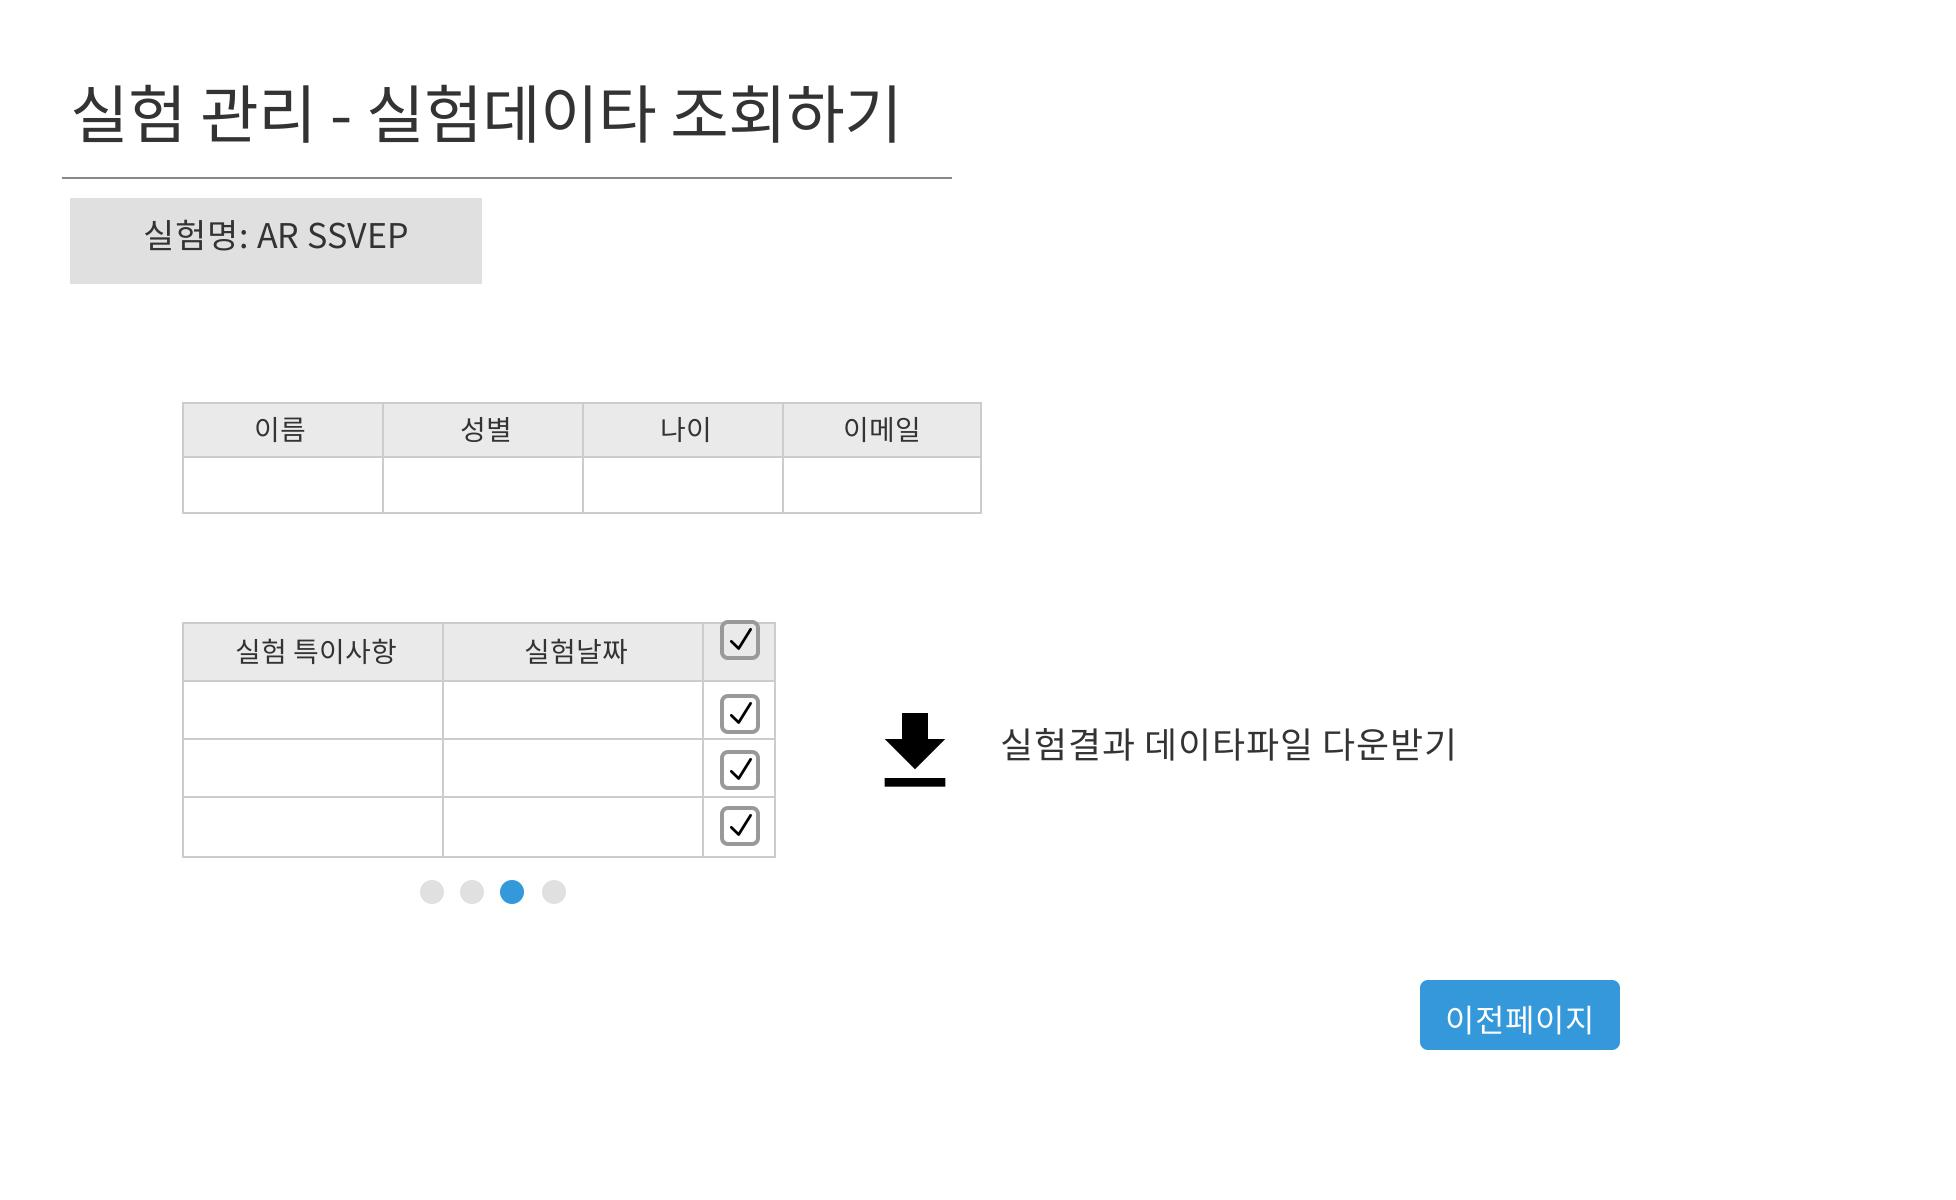
\includegraphics[width=0.5\textwidth,height = 7cm]{Oven_ver2/ver2]09_reviewingData.jpg}
If researcher select one of the applicants name and click the button for reviewing uploaded experiment result data, the above page will be shown.
\begin{itemize}
    \item A table which contains the conducted experiment organized in the order of date.
    \item Name, age, gender and email address of applicant.
    \item Button for downloading uploaded experiment result file.
\end{itemize}




 

\subsubsection{Uploading/Revising Experiment Result Data}

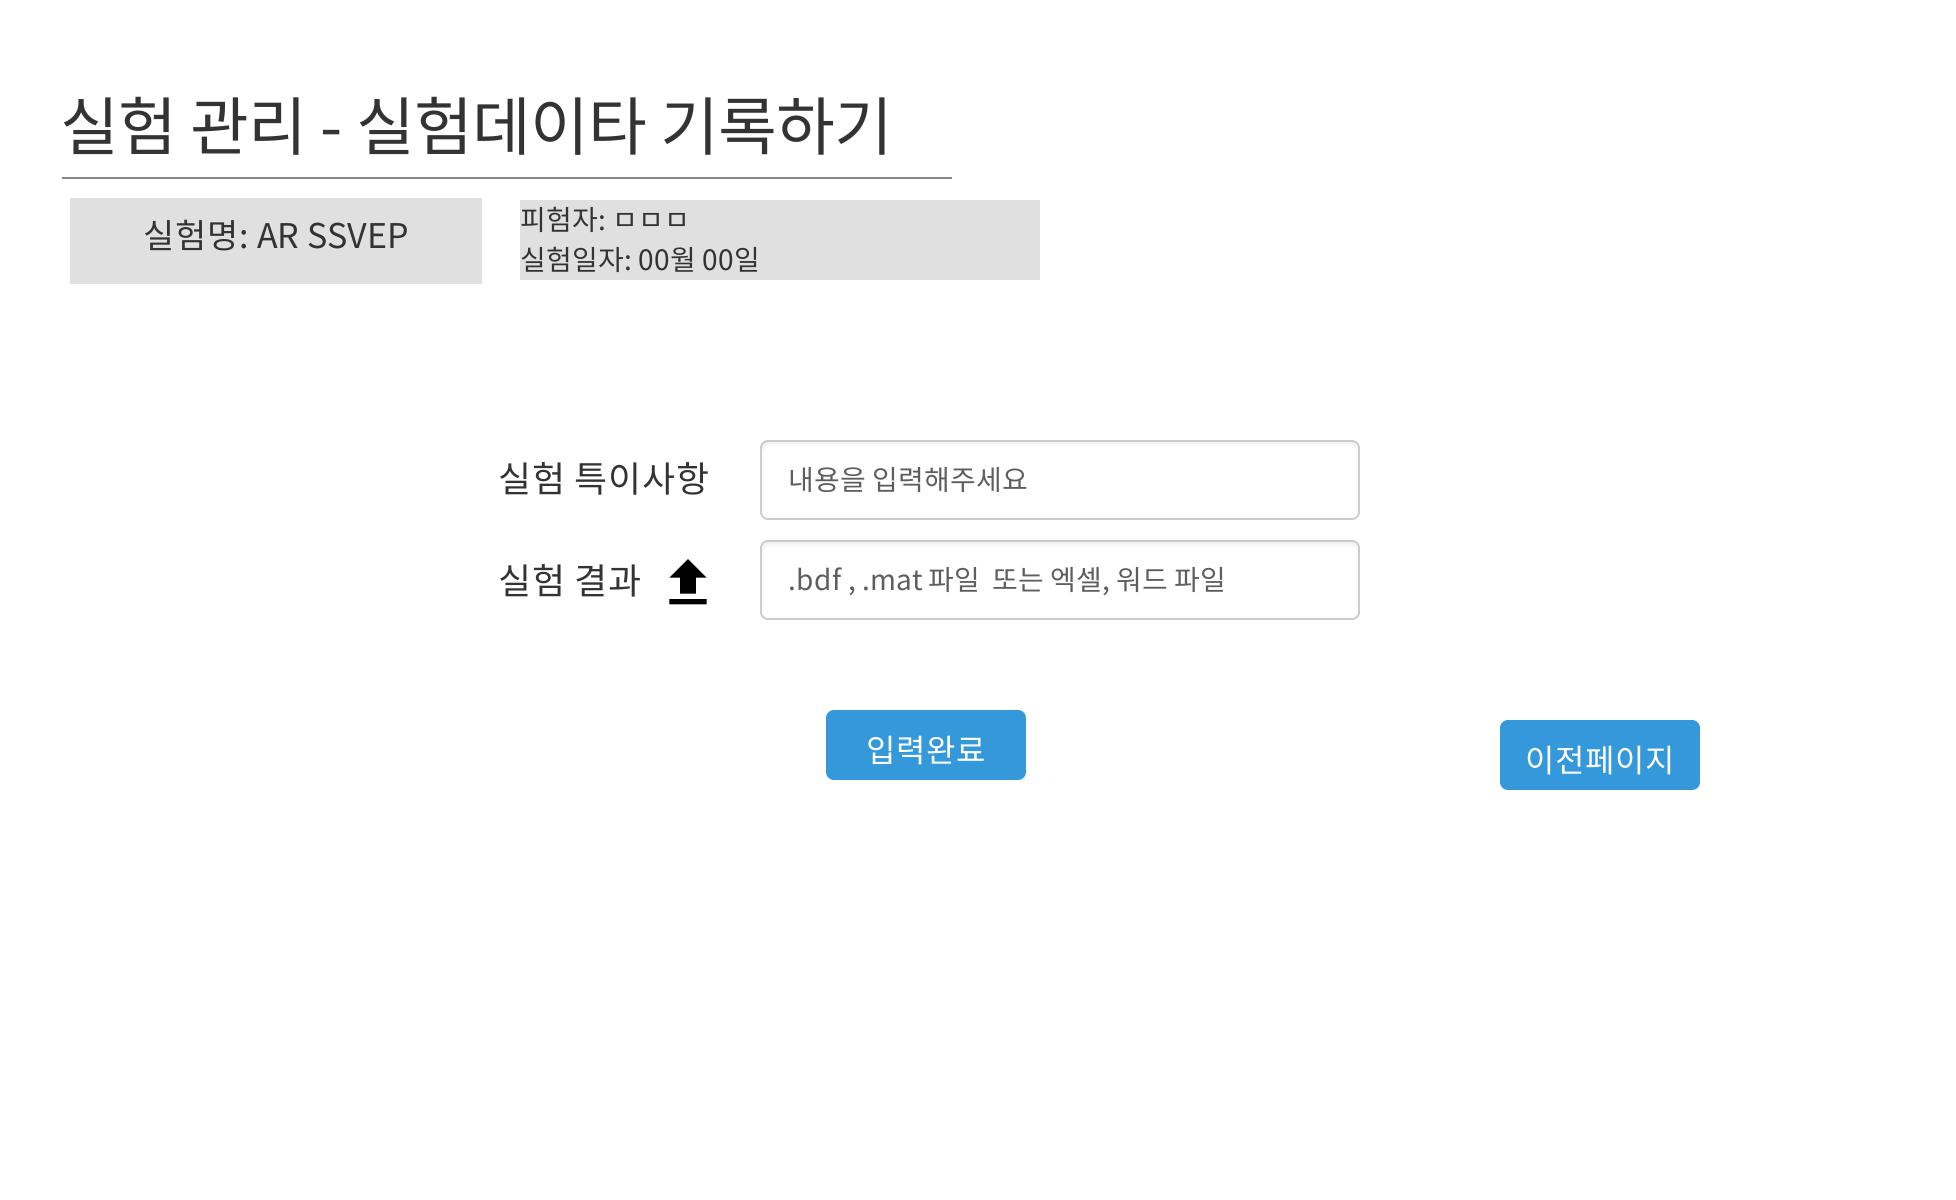
\includegraphics[width=0.5\textwidth,height = 7cm]{Oven_ver2/ver2]08_recordingData.jpg}
If researcher select one of the applicants name and click the button for uploading experiment result data, users can enter the specific features of applicants and upload the data file. 
\begin{itemize}
    \item Text bar for entering the special features of applicants
    \item Uploading bar
\end{itemize}


\subsubsection{New Experiment Schedule and Posting Recruitment Notice}
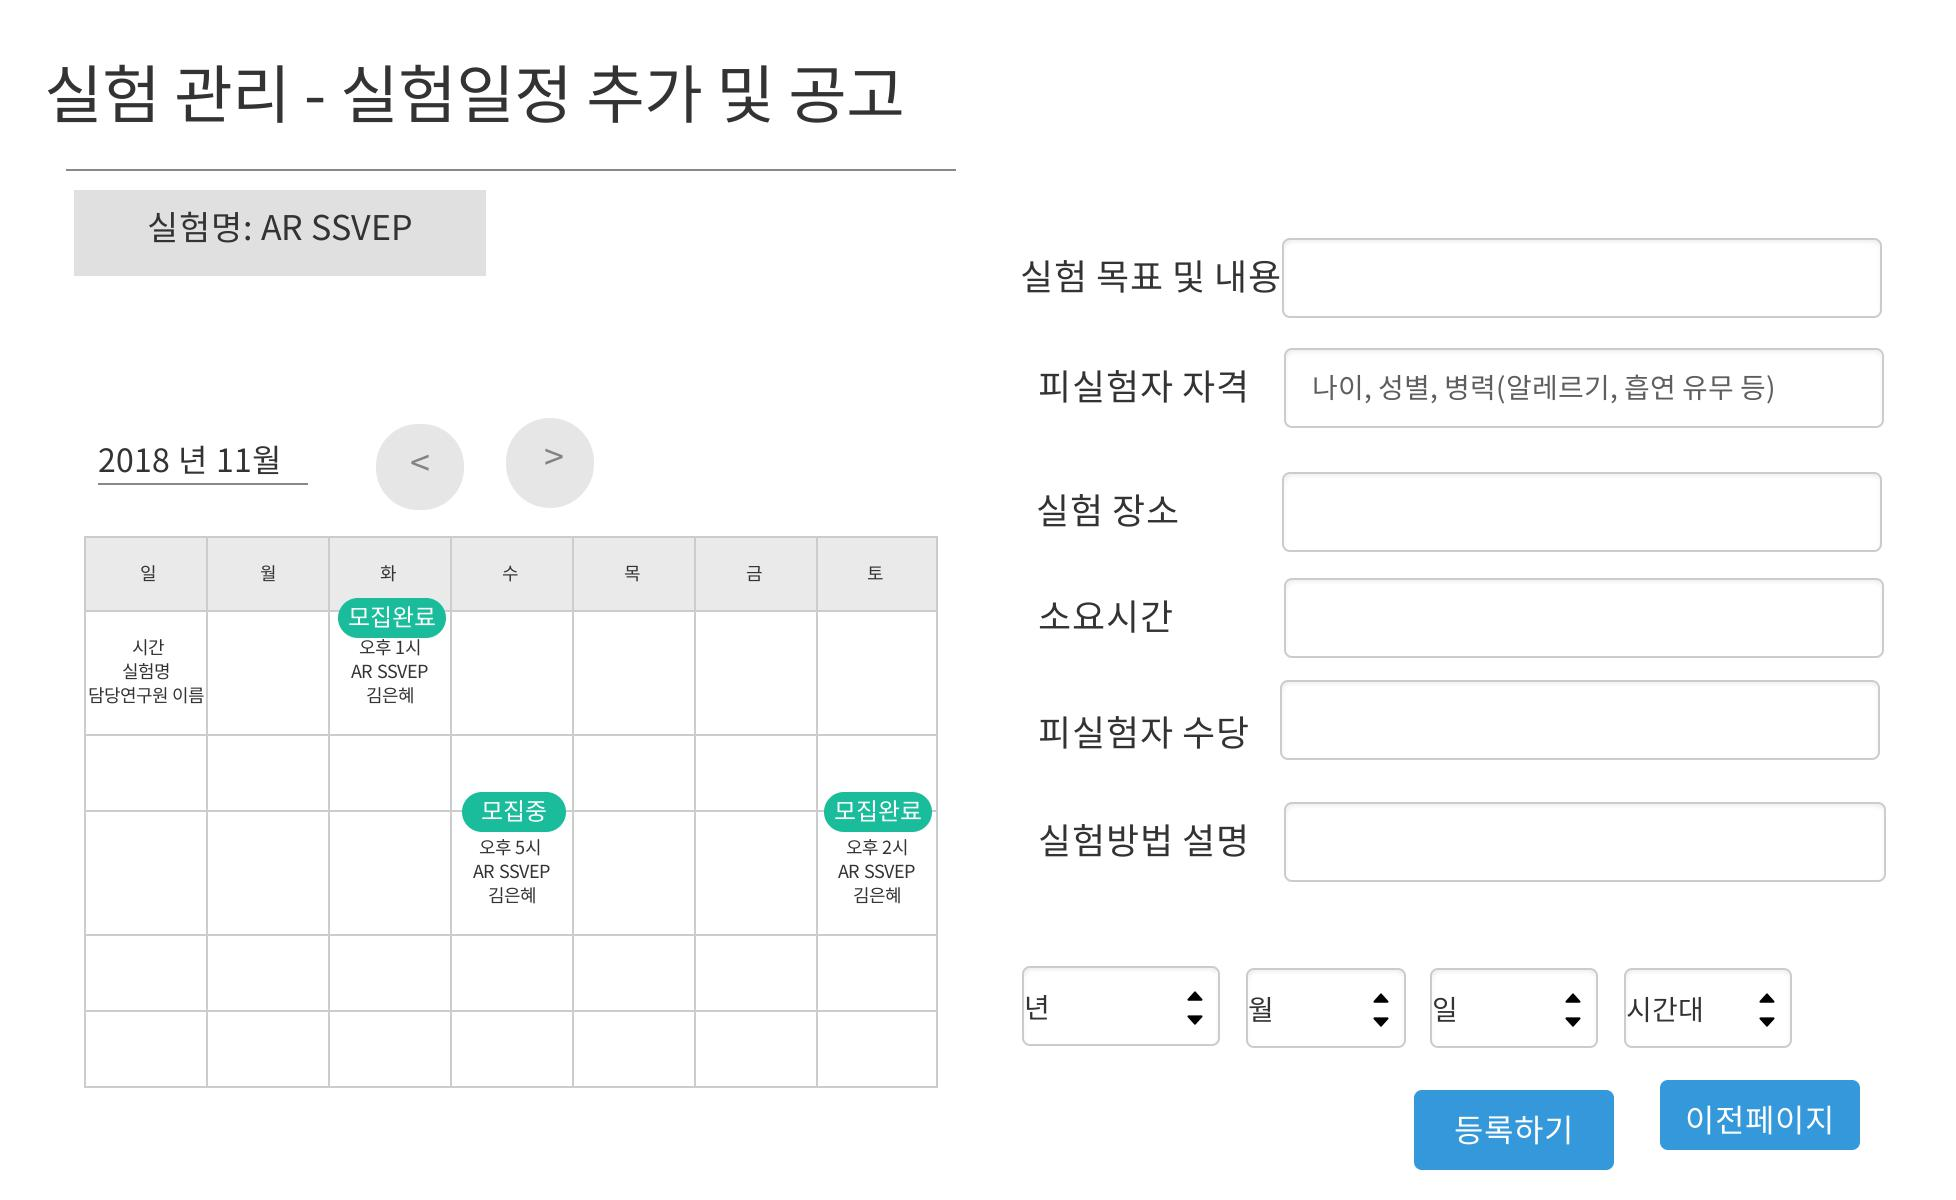
\includegraphics[width=0.5\textwidth,height = 7cm]{Oven_ver2/ver2]10_scheduleNotice.jpg}
The scheduled experiments will be shown in the form of calender. Lab researchers can choose the date and time to conduct experiment. They should type in the purpose of experiment, requirements for applicants, location, expected duration time, pay and the steps of experiment. All these information will instantly posted in the applicants' main page list in a well organized form as the button is clicked. 


\subsection{Functions For Applicants}
\subsubsection{Main Page\\}
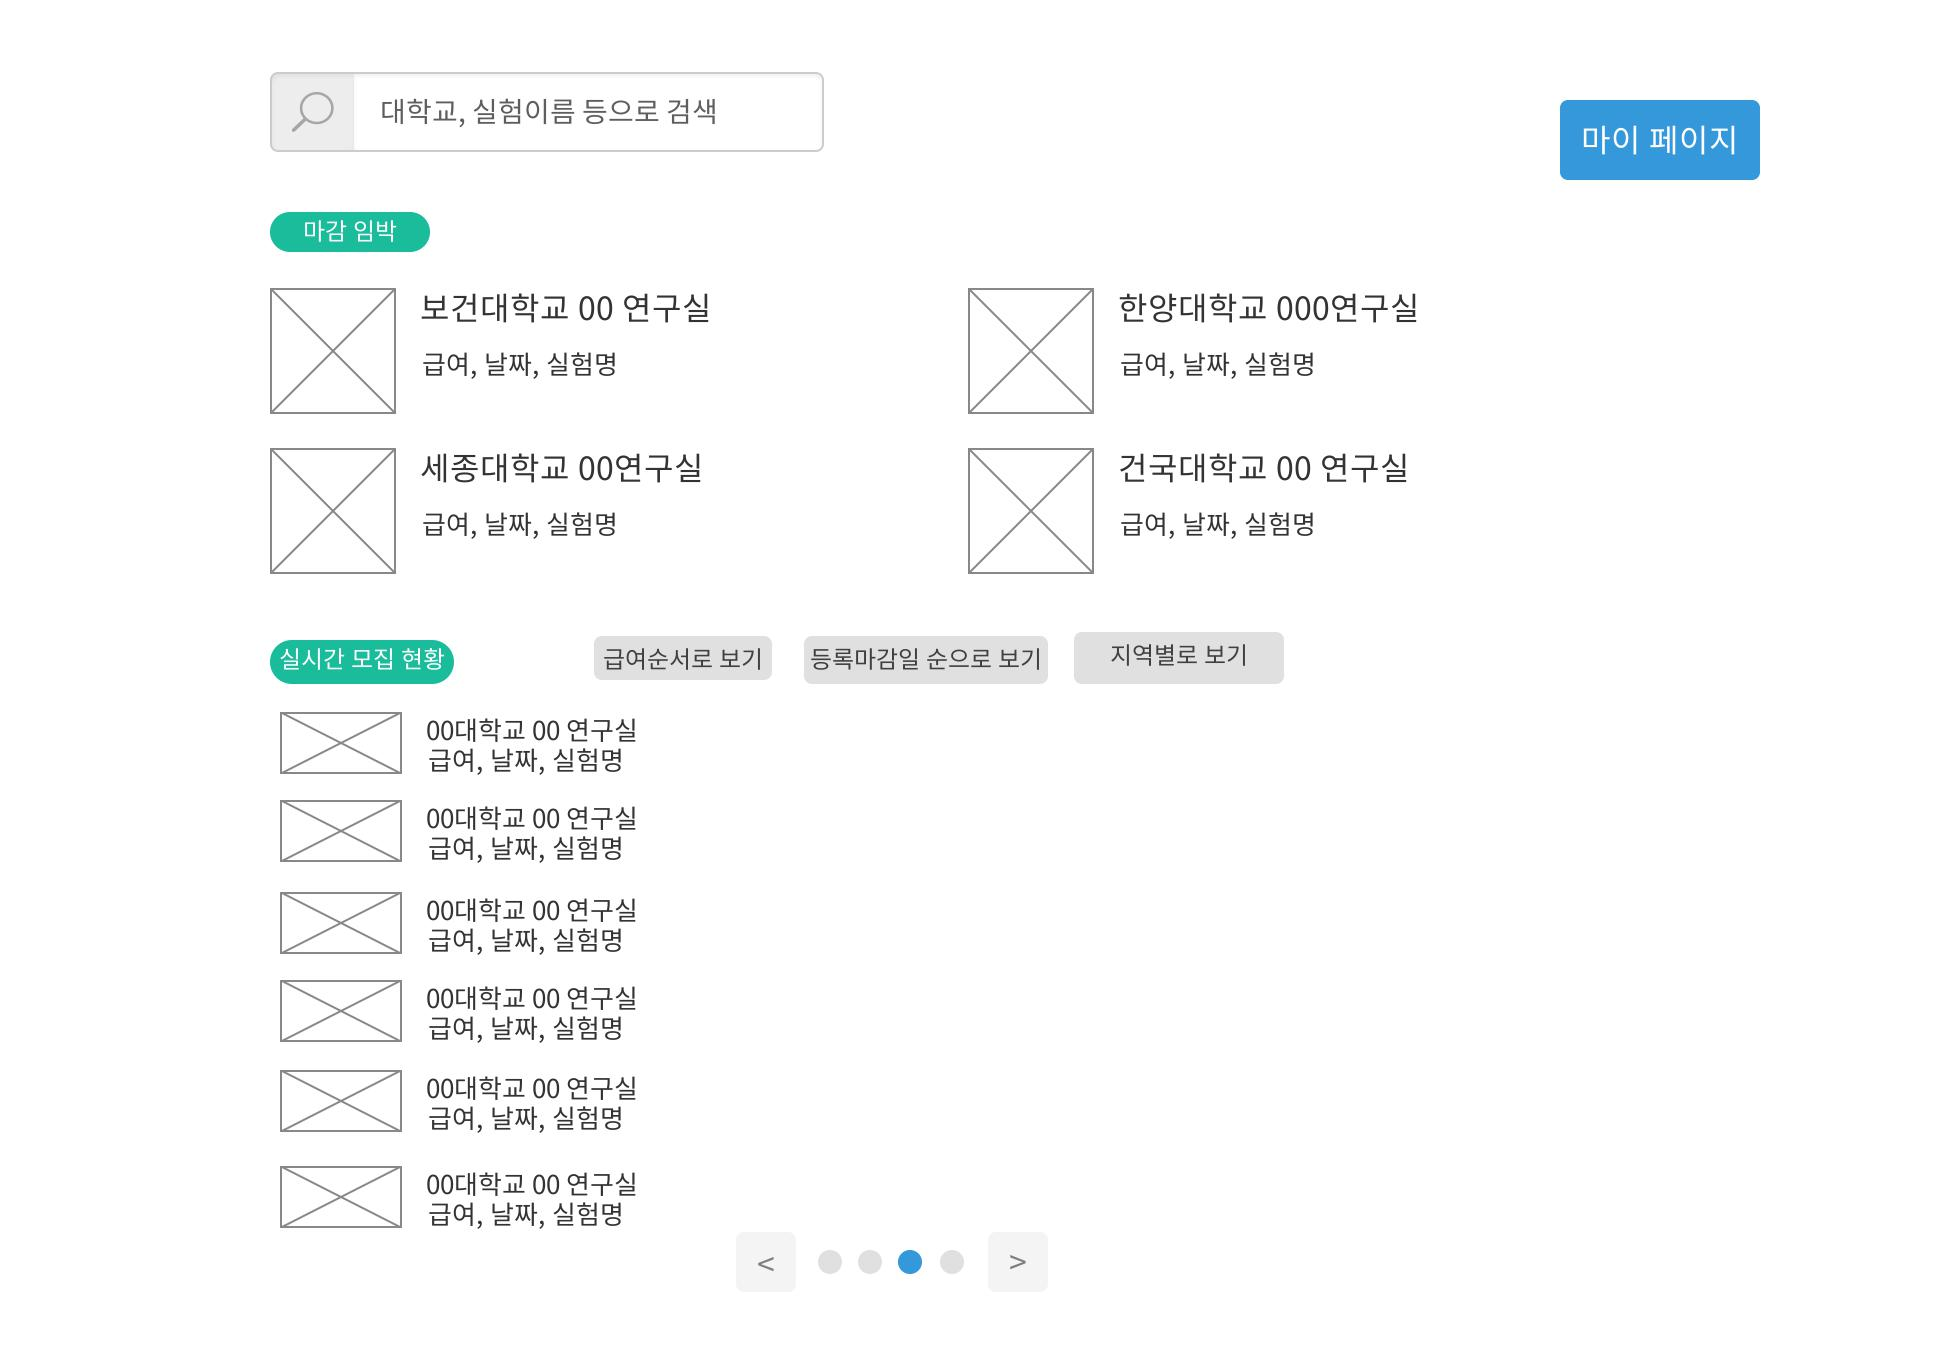
\includegraphics[width=0.5\textwidth,height = 8cm]{Oven_ver2/ver2]11_applicantMainPage.jpg}
Users can search for a specific experiment they prefer with key words like the name of experiment, related major or the name of university that the lab belongs to. At the top f list, recommended recruitment will be shown. Below this, the list of all the notices is located. This list is updated real time. If applicant click one of these elements, the page of Detailed Information Page will be shown. 



\subsubsection{Detailed Information Page}
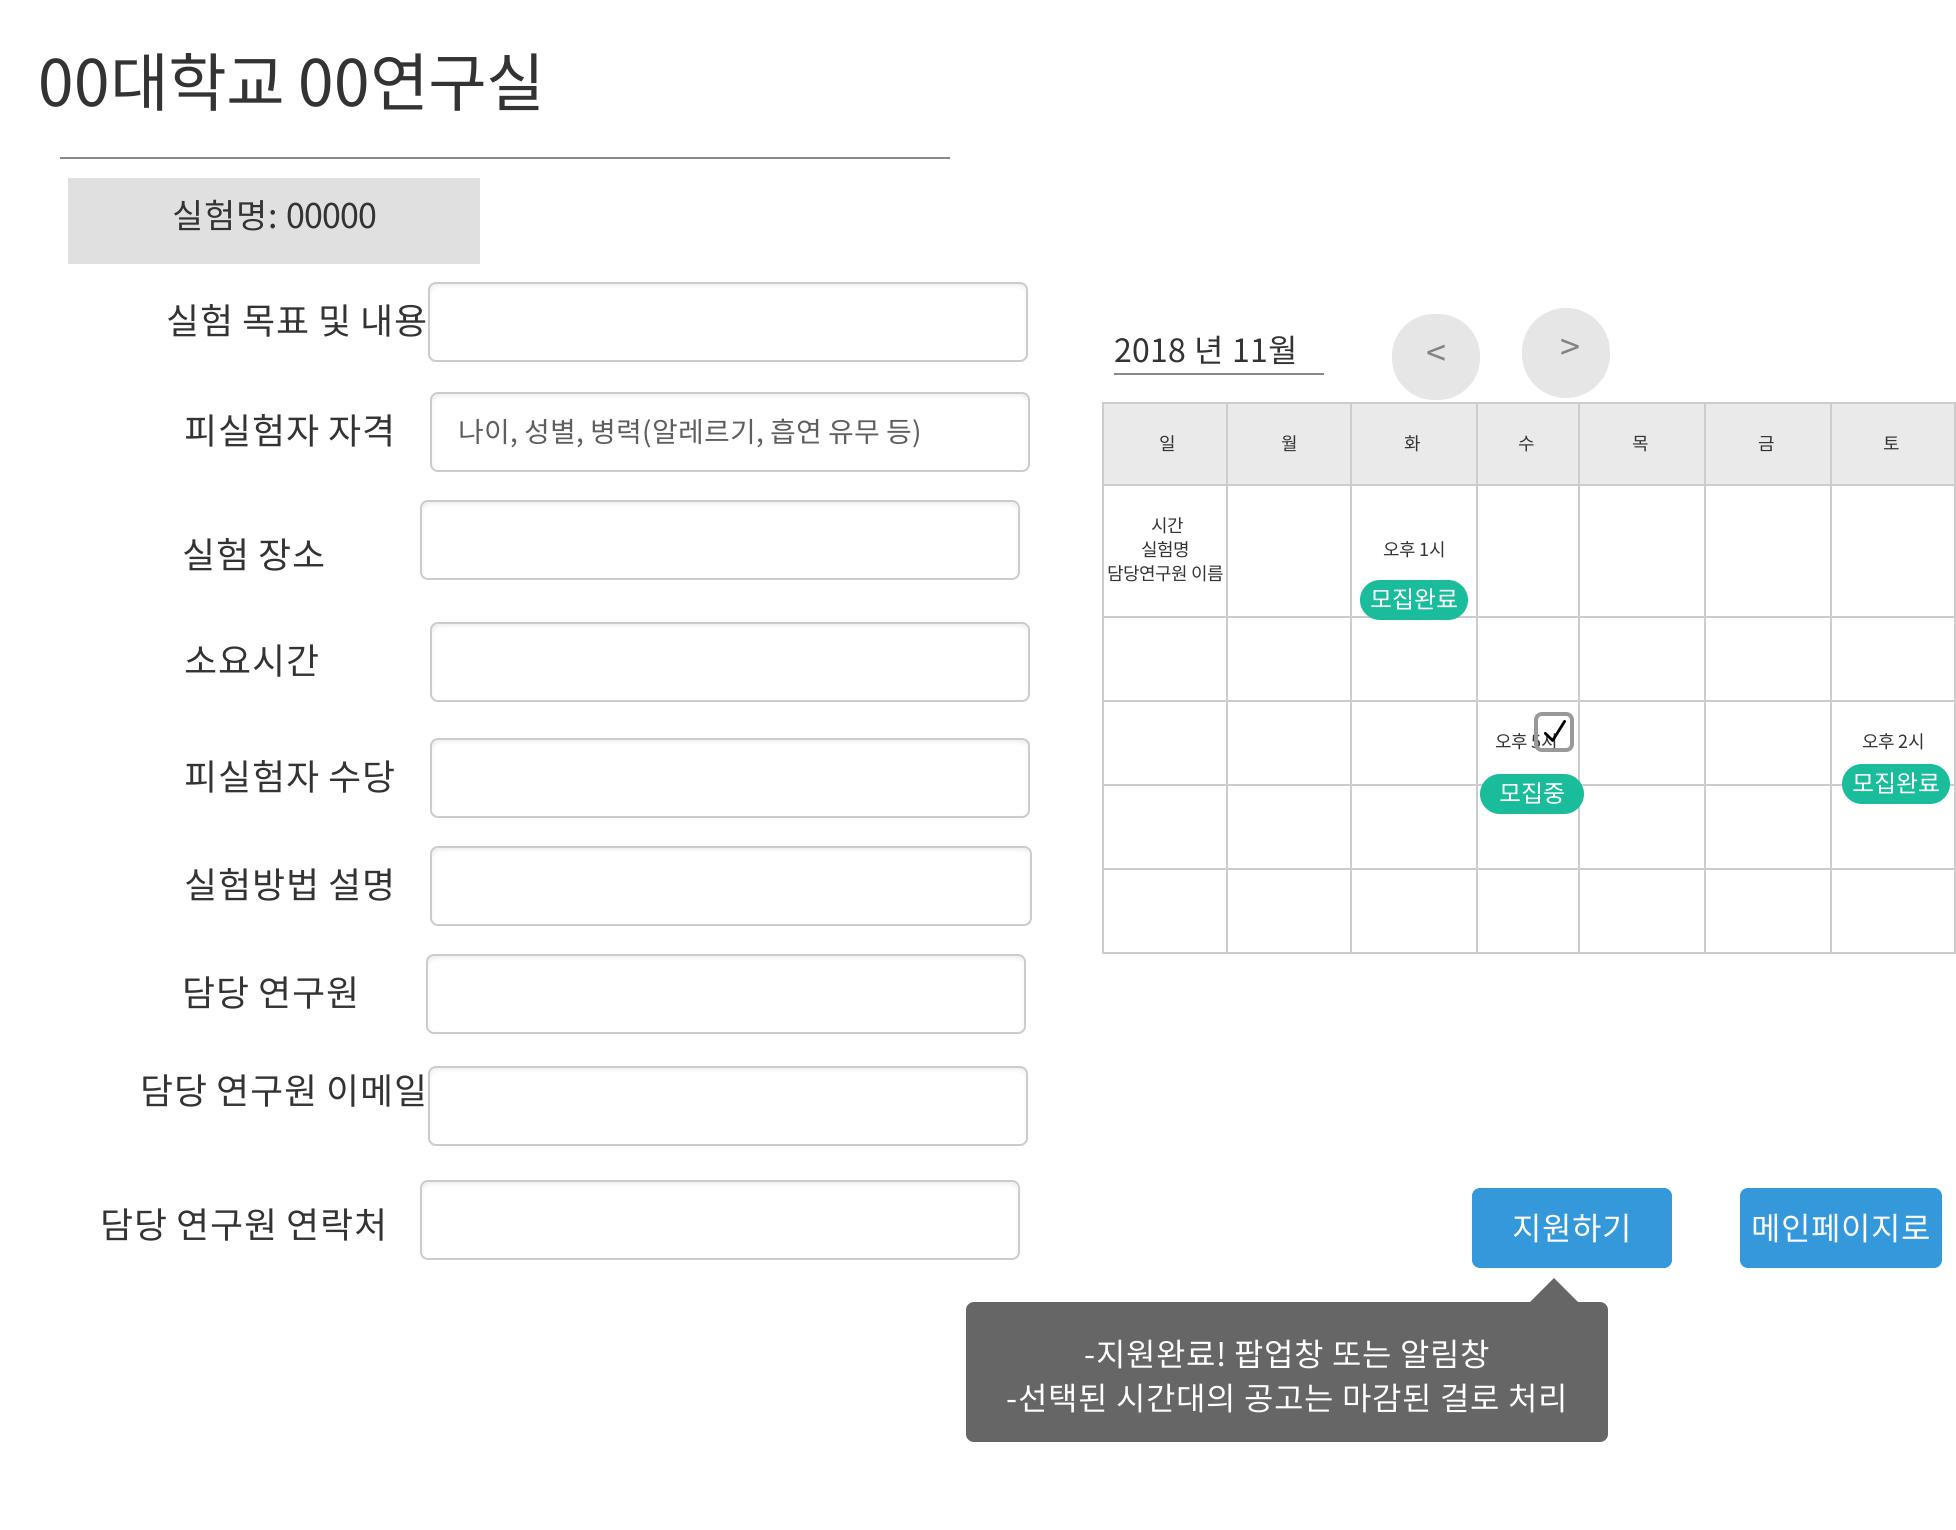
\includegraphics[width=0.5\textwidth,height = 7cm]{Oven_ver2/ver2]12_detailedExperimentPage.jpg}
Information of the experiment will be shown in the form as above image. Applicants should click a date and time then click the apply button. Their personal information which is entered at sign up phase will be transferred to lab. 

\begin{supertabular}{ |p{3cm}|p{4cm}| }
 \hline
 \multicolumn{2}{|c|}{Underlying Models and Operation} \\
 \hline
 Participant Model & When  User  apply for an experiment by clicking ’apply’ button, new Participant is created.  With this Participant Model, User’s data is connected to ExperimentDetails Model.\\
 \hline
 User Model & The account type of which who are willing to participate as applicants. \\
 \hline
\end{supertabular}

\subsubsection{Mypage For Applicant}
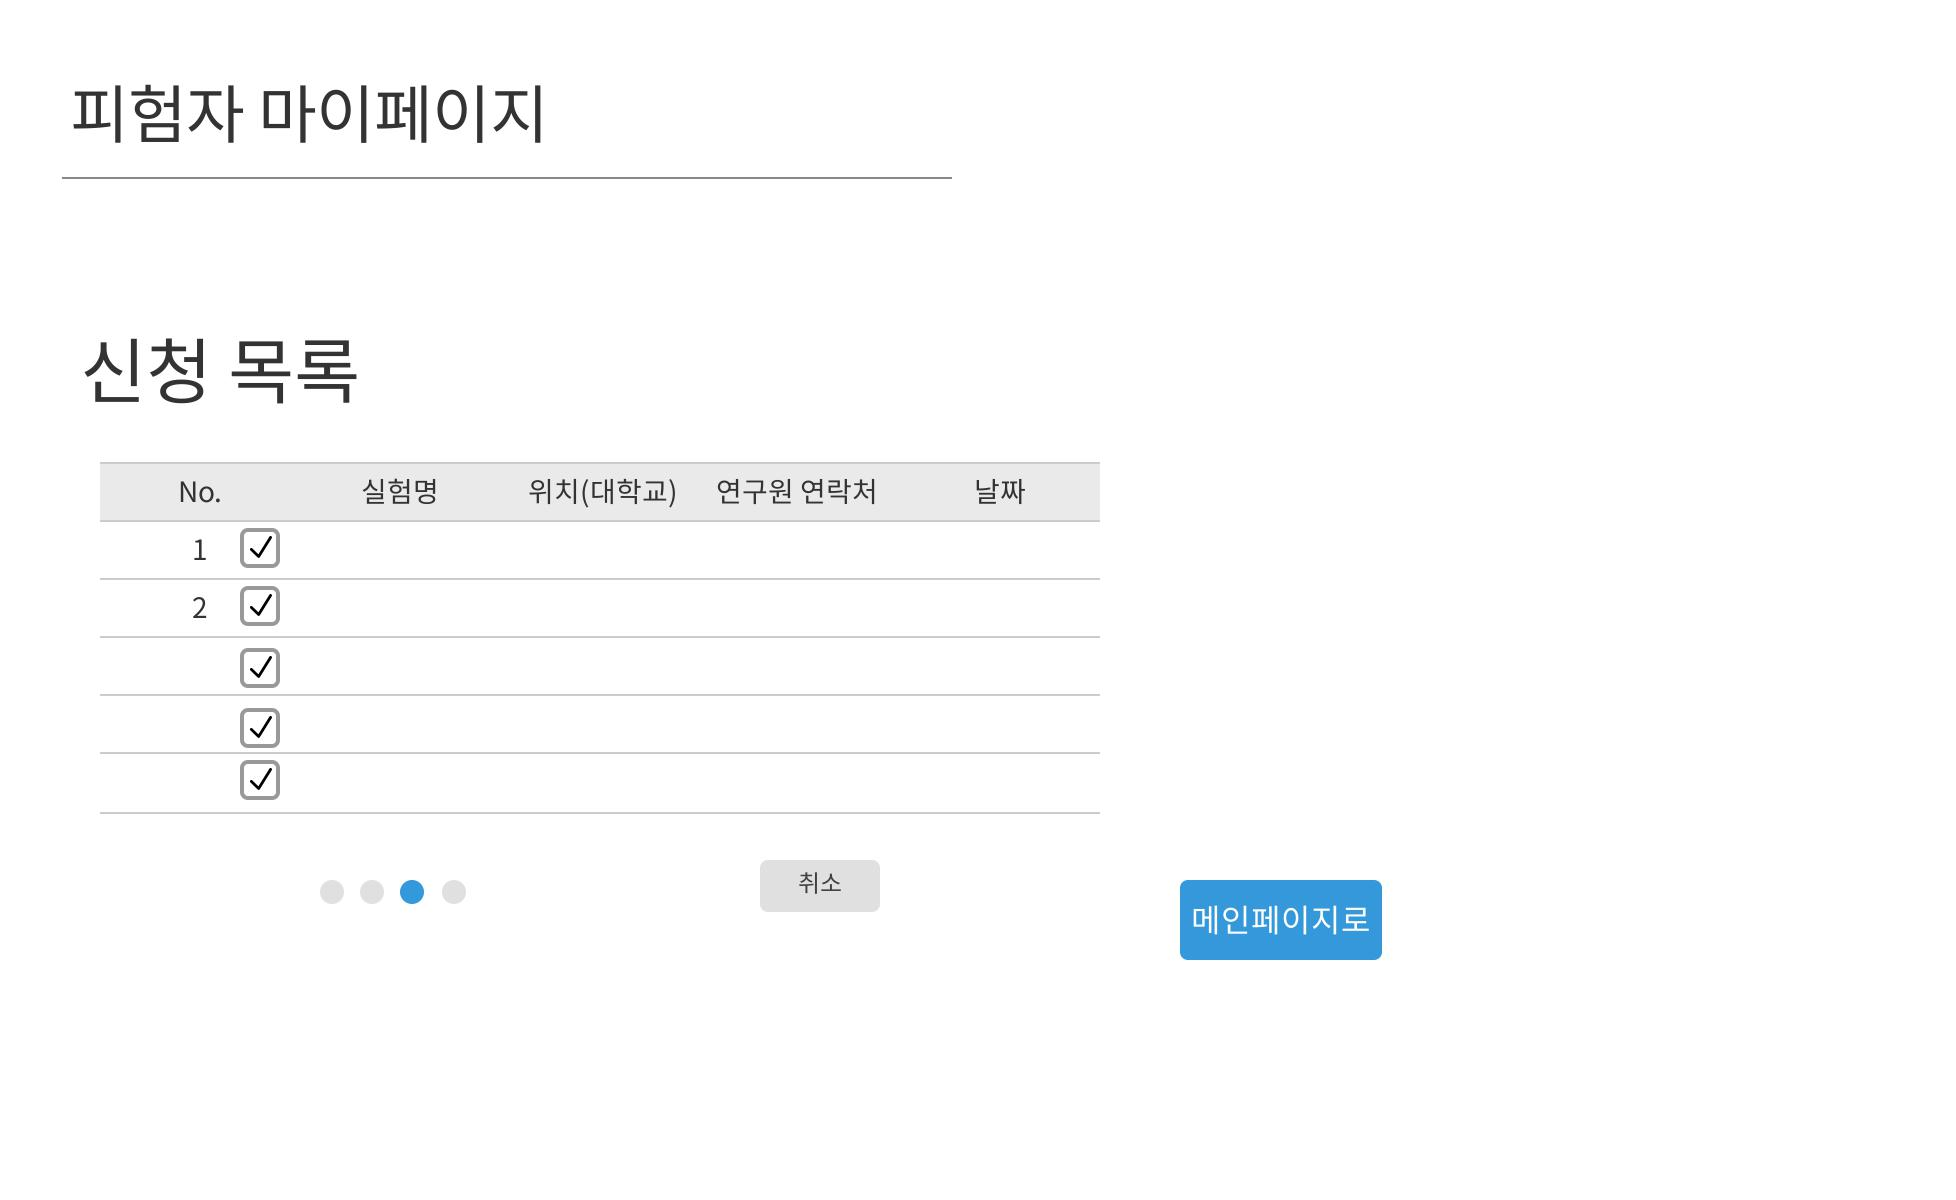
\includegraphics[width=0.5\textwidth,height = 8cm]{Oven_ver2/19_myPageForApplicant.jpg}
There is a list that contains all the experiments that applicant has applied for. They are organized in the order of the applying date. In the next column, applicant can see the name of experiment, location, contact of researcher in charge and the scheduled date. Click one of the elements, then the detailed information page will be shown.

\subsubsection{Information Page For Experiments In Mypage}
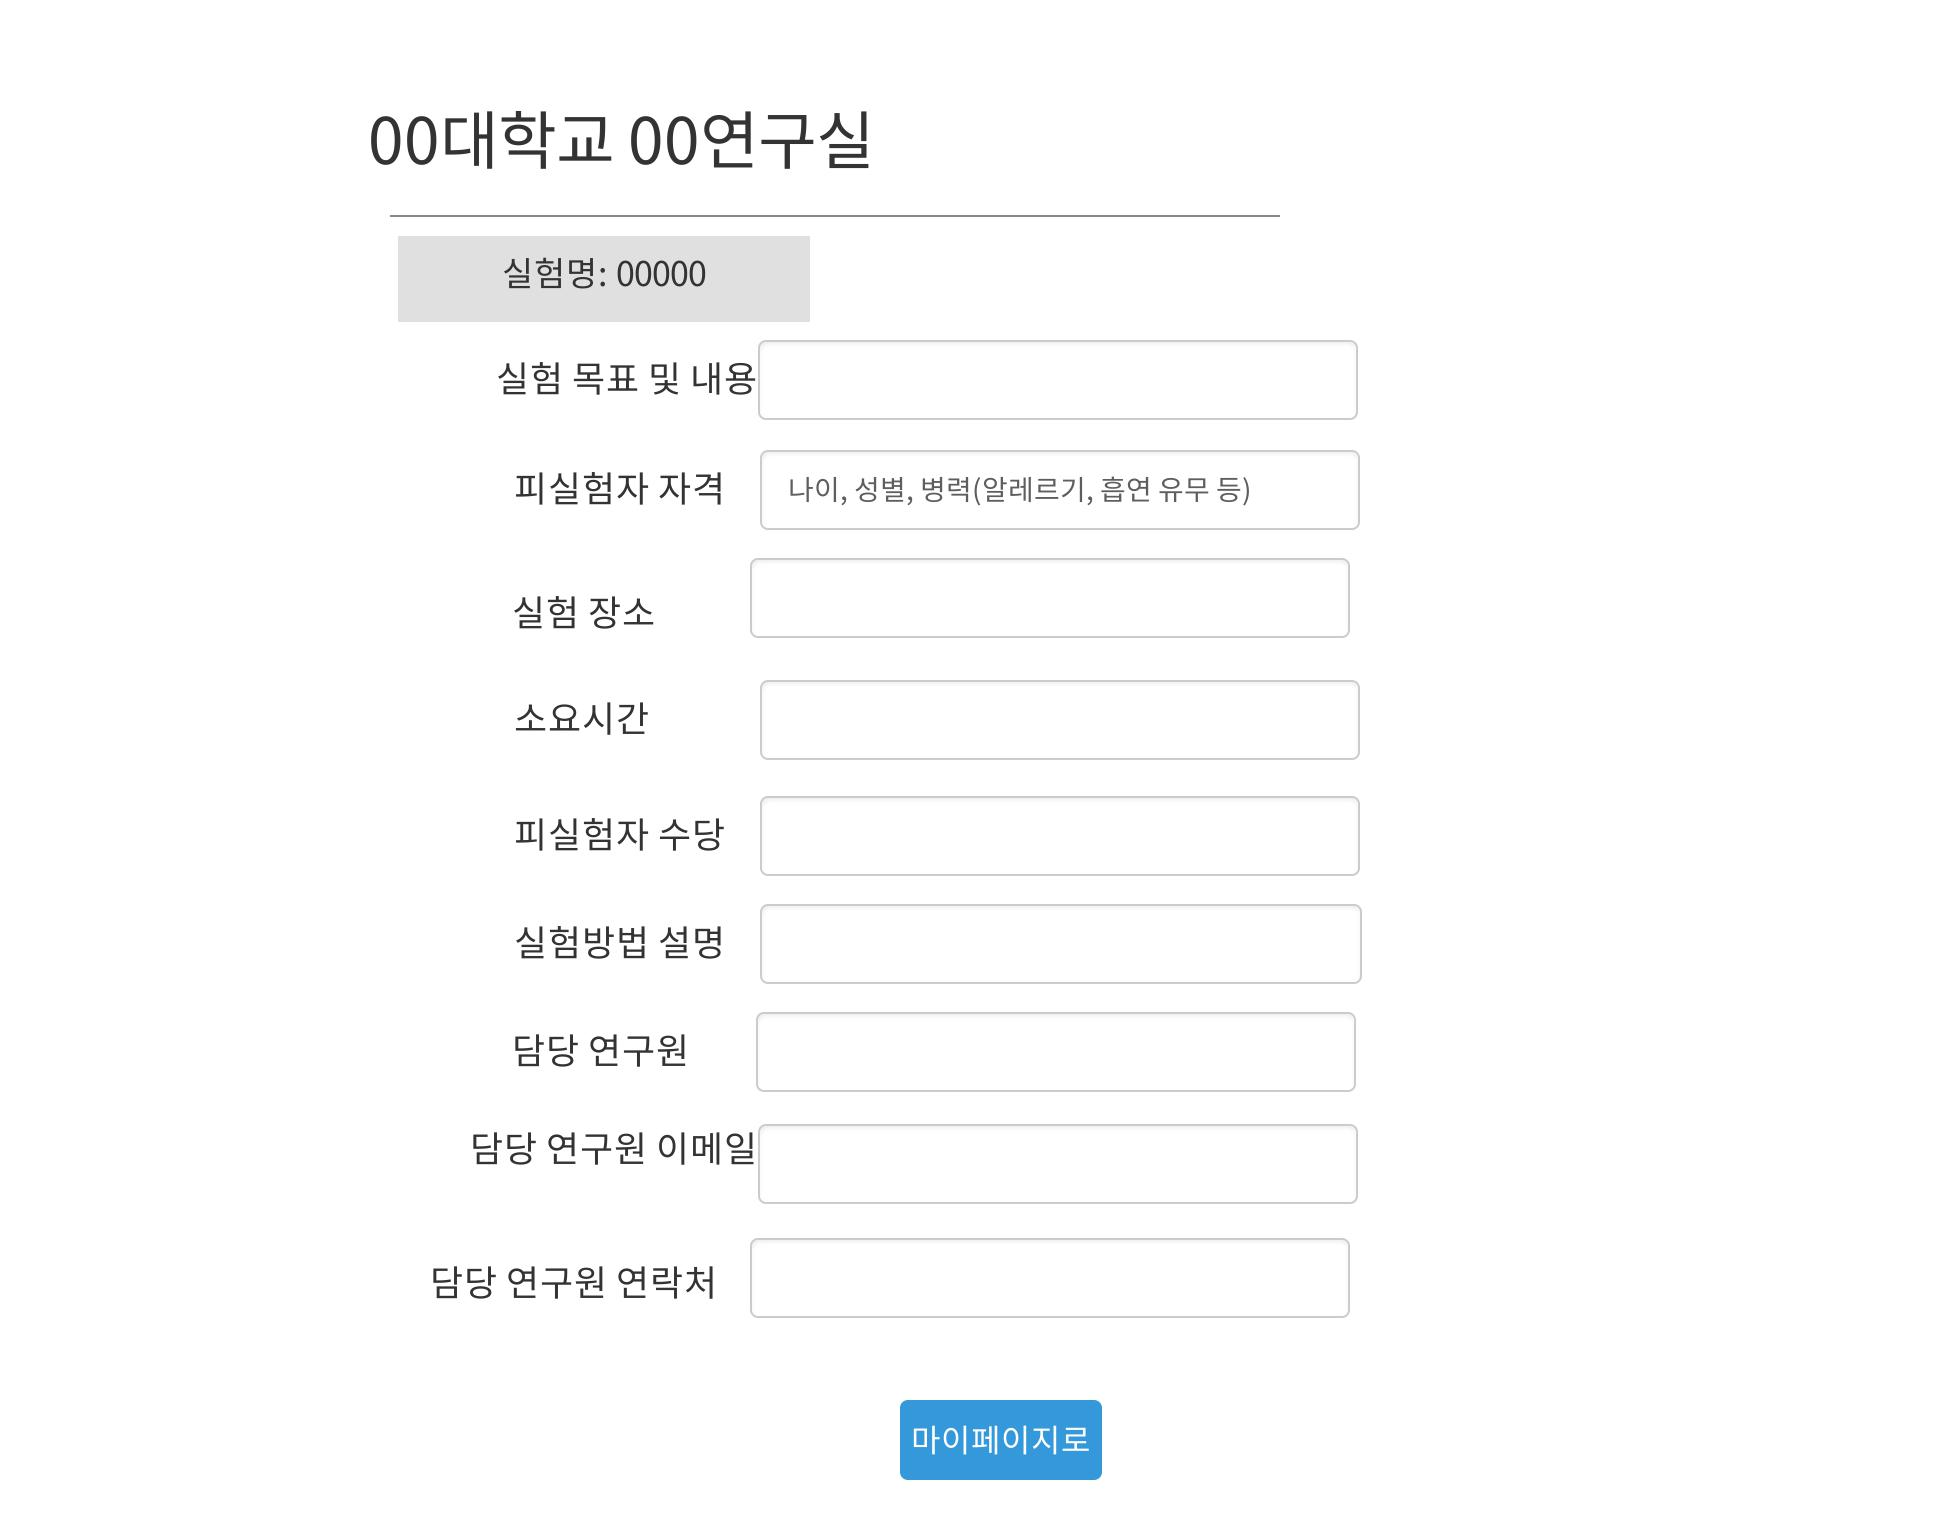
\includegraphics[width=0.5\textwidth,height = 8cm]{Oven_ver2/20_detailedInformationInMypage.jpg}




\section{Architecture Design Implementation }

\subsection{Overall Architecture}
\subsubsection{MVC pattern}
%%Actor Avatar%%
\begin{center}
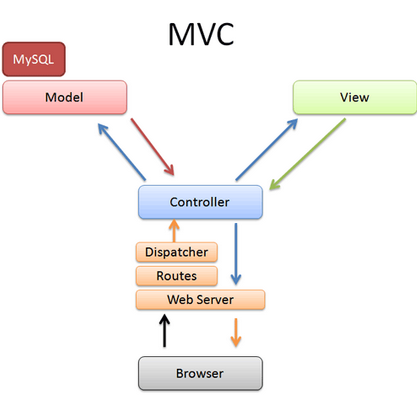
\includegraphics[width = 0.5\textwidth]{Architecture/MVC_structure.png}


\subsubsection{Model\\}
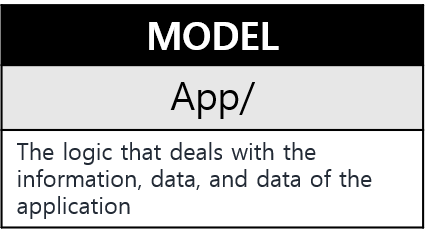
\includegraphics[width = 0.3\textwidth]{Architecture/Model.png}
\subsubsection{View\\}
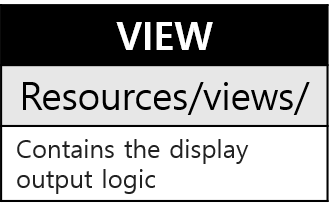
\includegraphics[width = 0.3\textwidth]{Architecture/View.png}
\subsubsection{Controller\\}
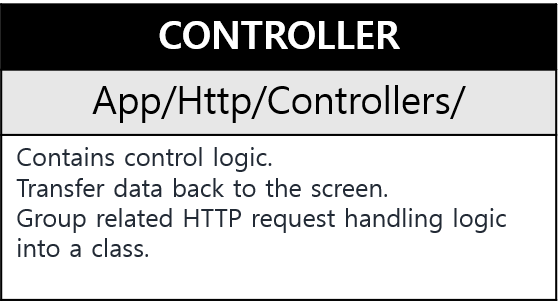
\includegraphics[width = 0.3\textwidth]{Architecture/Controller.png}
\subsubsection{Database\\}
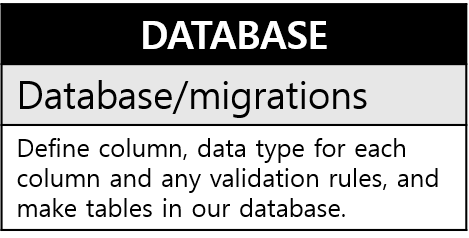
\includegraphics[width = 0.3\textwidth]{Architecture/Database.png}
\subsubsection{Router\\}
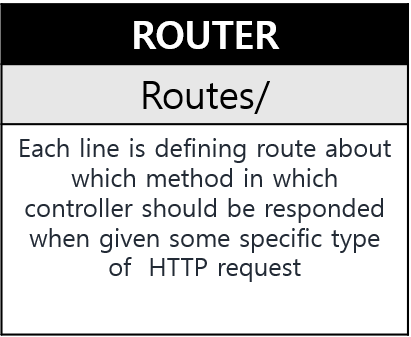
\includegraphics[width = 0.3\textwidth]{Architecture/Router.png}
\end{center}

\subsection{Relation Between Pages}
With the Kakao Oven prototyping tool, it is possible to test the web application almost same as the actual web application that our team has developed.\\
\textbf{Prototype link}\\https://ovenapp.io/view/bSZQZZQtyBhVFc5Ymd1DWZQ9O6uBGb58/Qybuc

\subsubsection{Link Of Sign Up and Sign In Pages\\}
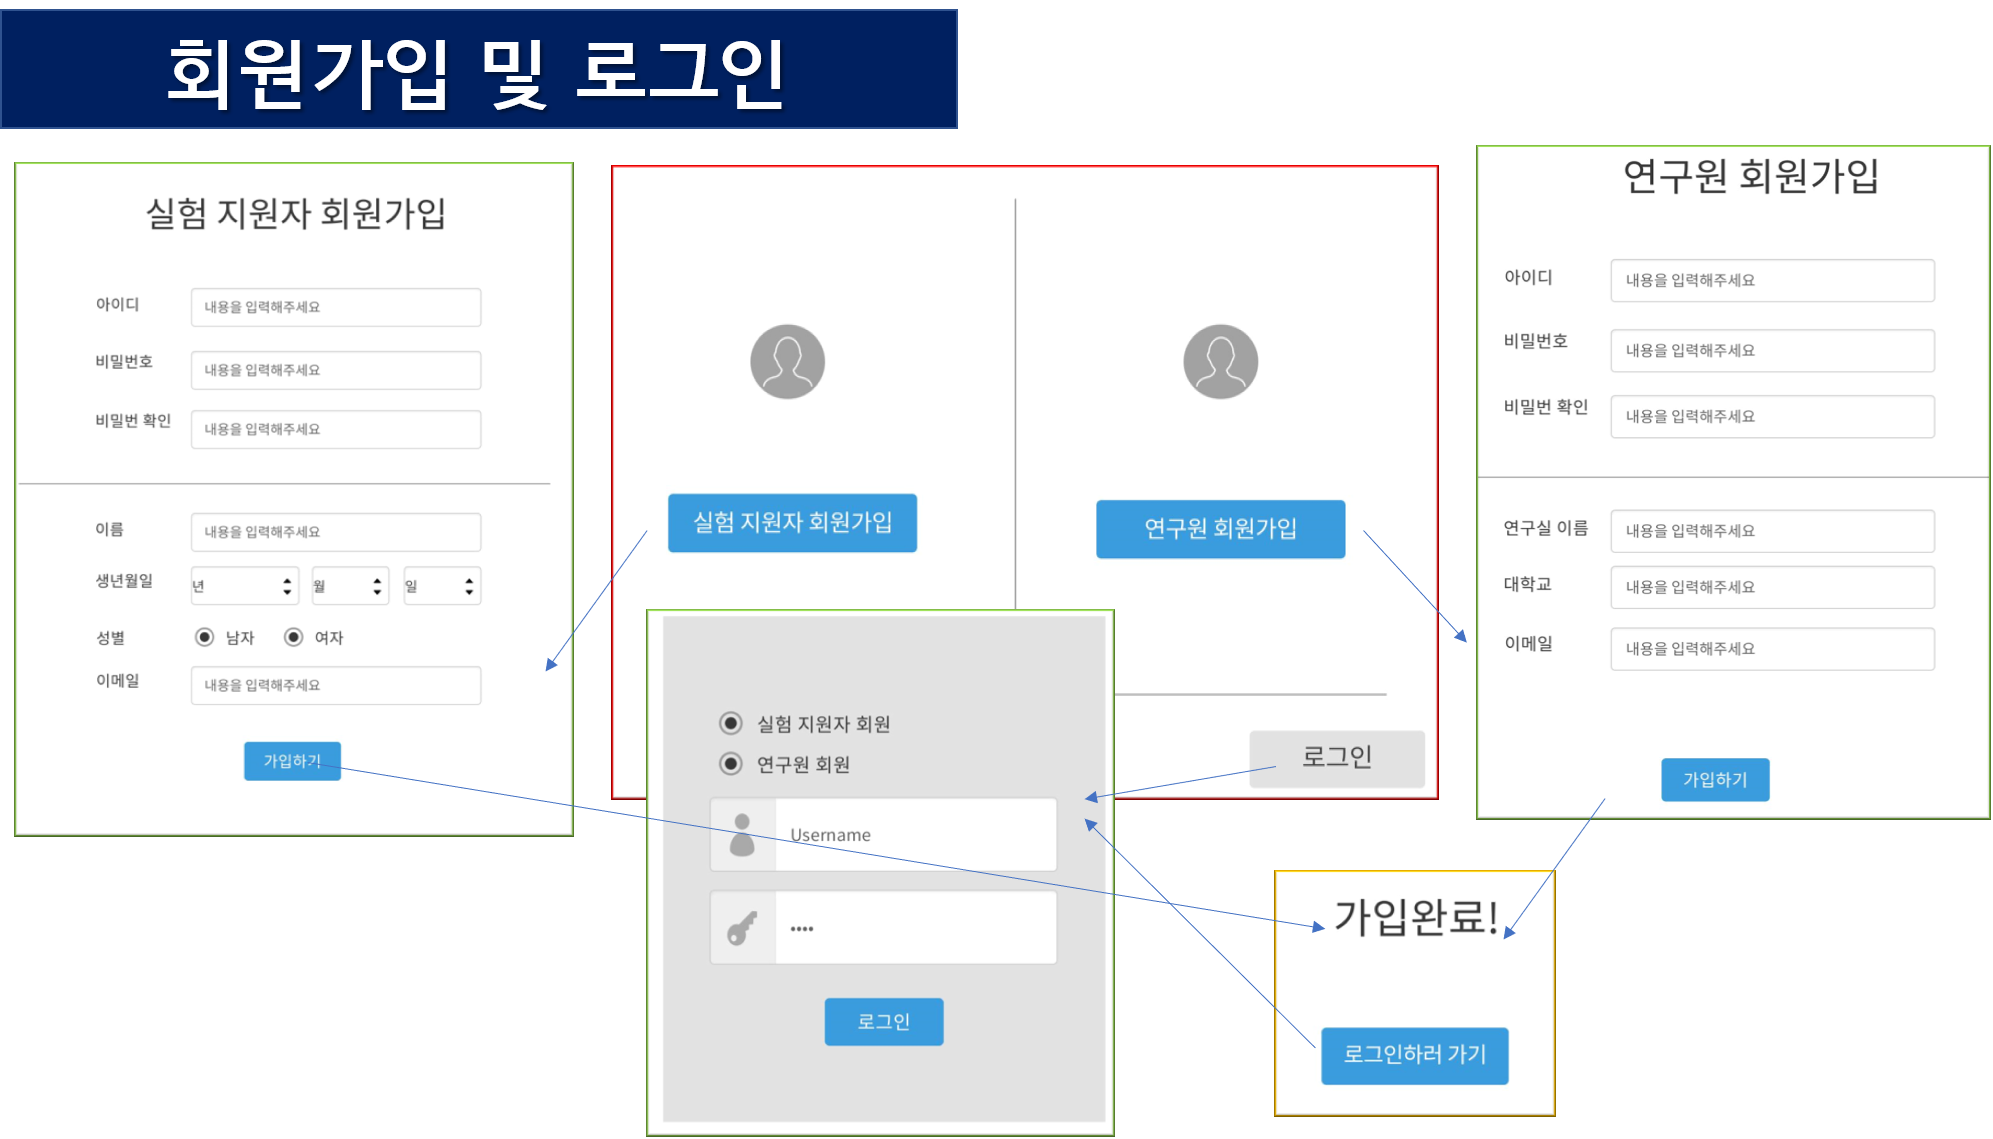
\includegraphics[width=0.5\textwidth,height = 7cm]{Oven/17_linkOfSignUpPages.png}



%\subsubsection{\\}
%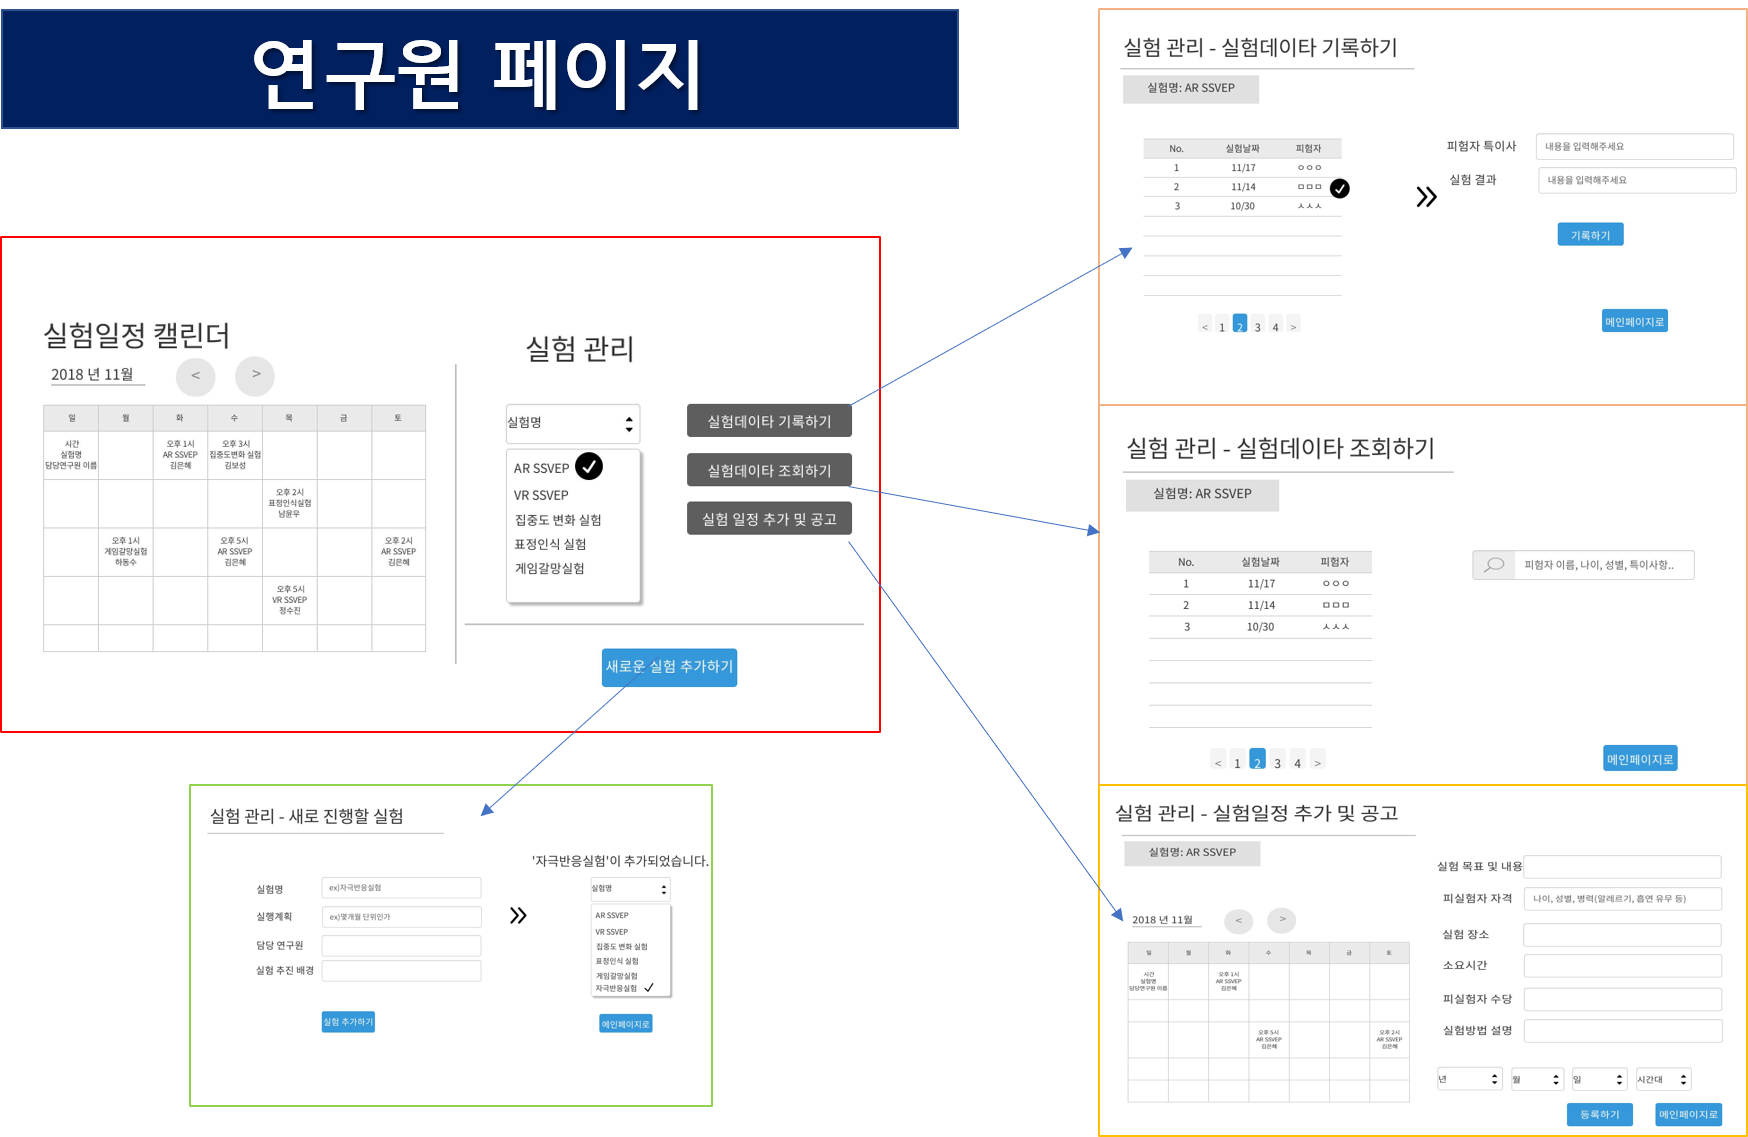
\includegraphics[width=0.5\textwidth,height = 7cm]{Oven/15_linkOfLabPages.png}

\subsubsection{Link Of Applicants' Pages\\}

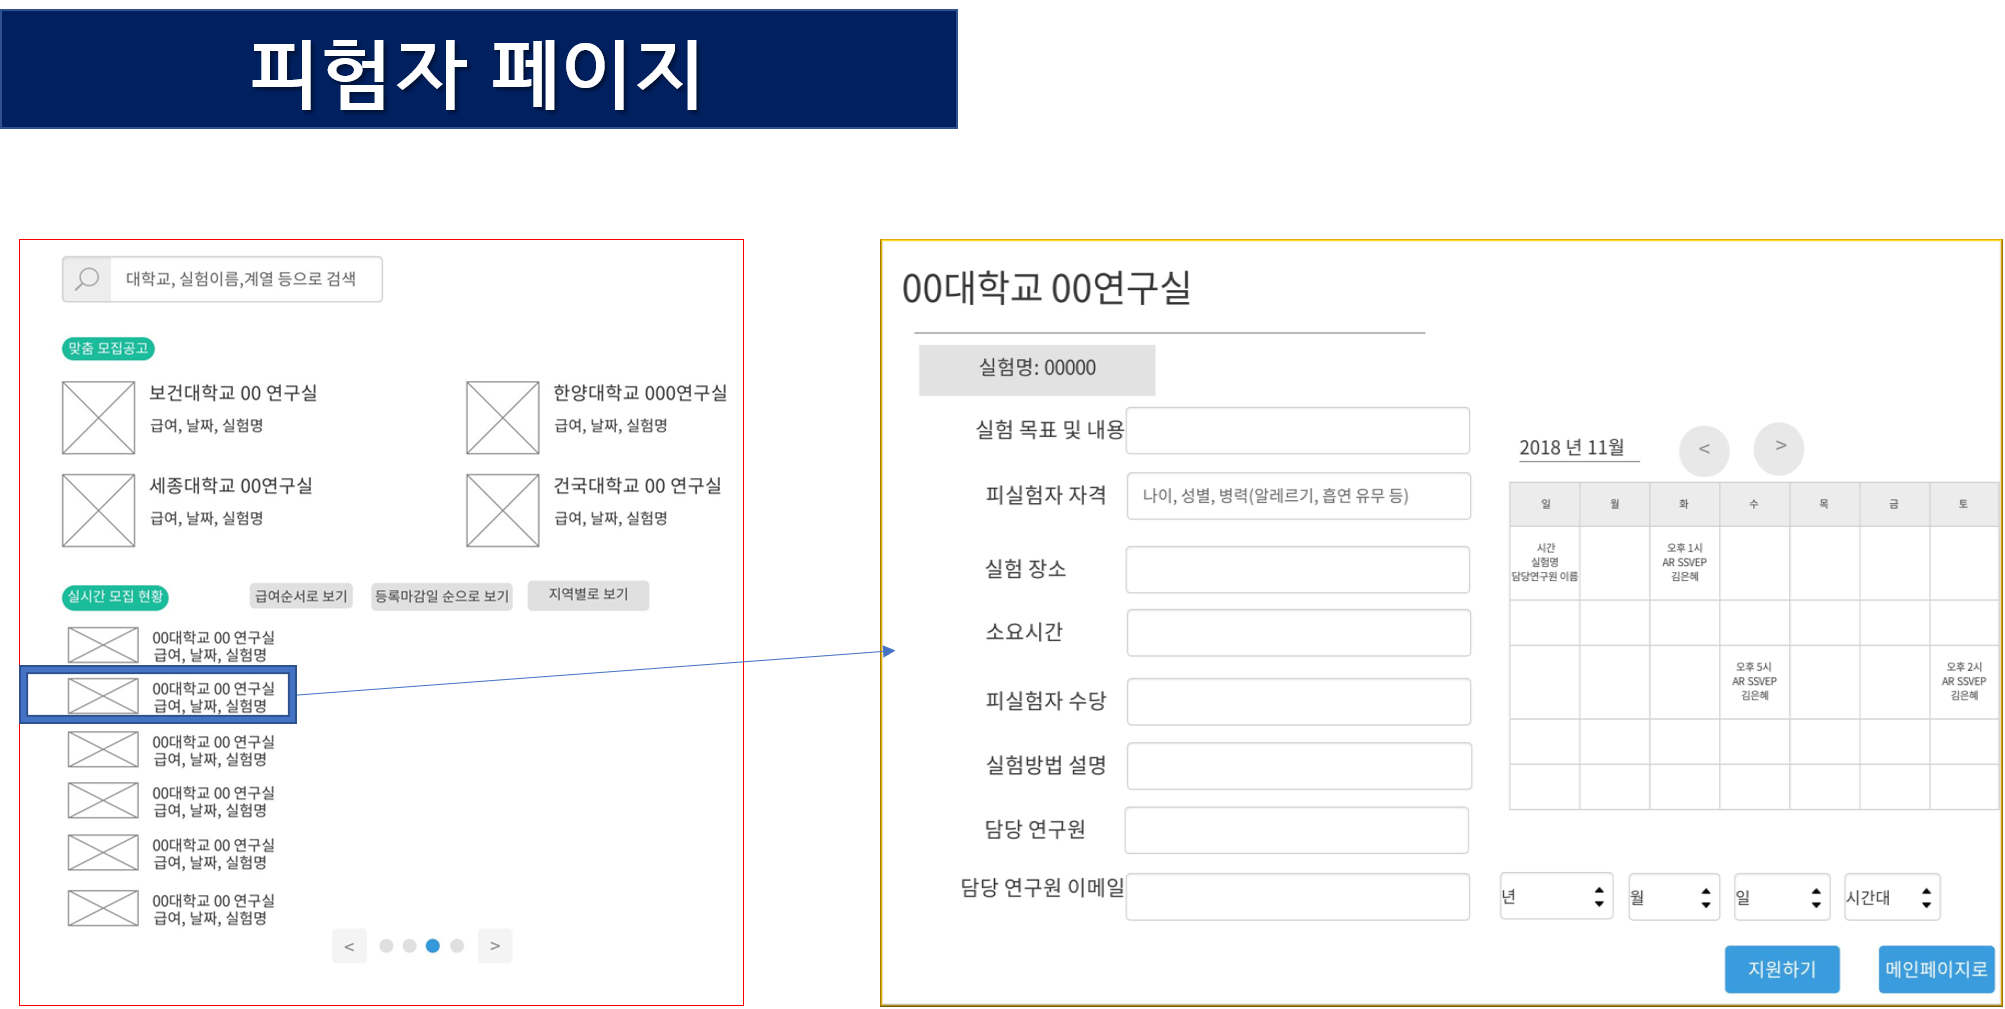
\includegraphics[width=0.5\textwidth,height = 7cm]{Oven/16_linkOfApplicantPages.png}

\subsection{Overall Modules Structure} %보성 워드문서 반영된 곳
In this section, the overall directory is visualized. Also, codes that have key role in our application are explained. \\
%%1.APP%%

\begin{center}
\begin{tikzpicture}

\begin{umlpackage}{App}

%\umlclass[template = 1]{Console}{}{}
\begin{umlpackage}{Console}
\end{umlpackage}
%\umlclass[x = 3,template = 2]{Exception}{}{}
\begin{umlpackage}[x=3]{Exception}
\end{umlpackage}
%\umlclass[x = 6, y = -3, template = 5]{Trivial Codes}{}{}

%\umlclass[y = -3,template = 3]{HTTP}{}{}
\begin{umlpackage}[y = -3]{HTTP}
\begin{umlpackage}{Controllers}
\end{umlpackage}
\begin{umlpackage}[x=3]{Middleware}
\end{umlpackage}
\begin{umlpackage}[x=3,y=-3]{Request}
\end{umlpackage}
%%\umlclass[x = 3, y = -3, template = 4]{Providers}{}{}
\begin{umlpackage}[y = -3]{Providers}
\end{umlpackage}

\end{umlpackage}




\end{umlpackage}

\end{tikzpicture}
\end{center}
\subsubsection{App/Console\\}
\begin{itemize}
    \item Console/Kernel.php: class kernel is responsible for specifying which custom commands should be made available to users and when to automatically execute various commands and tasks (by using the task scheduler).\\
    
\end{itemize}
\subsubsection{App/Exception\\}
\begin{itemize}
    \item Exceptions/Handler.php: class Handler is where all exceptions triggered by your application are logged and then rendered back to the user.
    \\\textit{report()} is the method used to log exceptions or send them to an external service. The report method passes the exception to the base class where the exception is logged
    \\\textit{render()} is the method responsible for converting a given exception into an HTTP response that should be sent back to the browser. By default, the exception is passed to the base class which generates a response for you.\\
\end{itemize}
\subsubsection{App/Http/Controllers/Admin\\}




\begin{itemize}
    \item AdminSearchController.php: search around Experiment\_Result model and Experiment\_Details model.
    \item ExperimentDetailsController.php: Let admins search, read, create, store, edit, update, delete data by using ExperimentDetails Model.
    \item ExperimentController.php : Let admins search, read, create, store, edit, update, delete data by using Experiment Model.
    \item ExperimentResultController.php: Let admins search, read, create, store, edit, update, delete data by using ExperimentResult Model.\\
\end{itemize}
\subsubsection{App/Http/Controllers/user\\}
\begin{itemize}
    \item UserHomeController.php: Show the latest data among experimentdetails model and let users check if there is new experimentdetails data and their detailed information.
    \item UserMyPageController.php: Show what experiments users applied for and let them cancel the application. By using Auth::check function to check who is currently logged in and get the information about the logged in user, we can bring the data from Participants Model, which has the two foreign keys that correspond to User’s id and ExperimentDetails’ id, respectively.\\
\end{itemize}
\subsubsection{App/Http/Middleware\\}
\begin{itemize}
    \item Authenticate.php: Get the path the user should be redirected to if they are not logged in.
    \item RedirectIfAuthenticated.php: Handle an incoming request. Two redirecting routes for user and admin.\\
\end{itemize}
\subsubsection{App/Http/Providers\\}
\begin{itemize}
    \item AuthServiceProvider.php: Determine if a user is authorized to perform a given action.\\
\end{itemize}
\subsubsection{App/Http/Requests\\}
\begin{itemize}
    \item ResultRequest.php:It contains validation rules for each field that apply to the request thrown by admin when they create, edit, update, store result for the experiment.
    \item UploadRequest.php: It contains validation rules for each field that apply to the request thrown by admin when they create, edit, update, store new recruitment for experiment.\\
\end{itemize}
\subsubsection{Models}
Models are located at App/. Roughly, there are two types of accounts. Researcher and applicant. Admin Model handles researcher's account and User Model handles applicant's account. 
\begin{itemize}
    \item Admin Model (Admin.php) allow us to fluently query the database table associated with the Admin model, as well as insert new records into the Admin table.
    \item Participant Model (Participant.php): When User apply for an experiment by clicking 'apply' button, new Participant is created. With this Participant Model, User's data is connected to Experiment\_Details Model. 
\end{itemize}
\subsubsection{Kernel.php}
This file is located at App/Http/. It contains application route middleware groups and application’s global HTTP middleware stack that are run during every request to application.\\


%%2.BOOTSTRAP%%
\begin{center}
\begin{tikzpicture}

\begin{umlpackage}{Bootstrap}

\begin{umlpackage}{Cache}

\end{umlpackage}

\end{umlpackage}

\end{tikzpicture}
\end{center}
\subsubsection{Bootstrap/Cache\\}
Contain information about binding the important interfaces and returning the application instance.\\

%%3.CONFIG%%
\begin{center}
\begin{tikzpicture}

\begin{umlpackage}{Config}

\end{umlpackage}

\end{tikzpicture}
\end{center}
\subsubsection{Config\\}
It contains basic functions of Laravel framework, and defines how each system works.\\

%%4.DATABASE%%

\begin{center}
\begin{tikzpicture}

\begin{umlpackage}{Database}
%\umlclass[template = 1]{Factories}{}{}
\begin{umlpackage}[x=2.5]{Factories}
\end{umlpackage}
%\umlclass[x = 3,template = 2]{Migrations}{}{}
\begin{umlpackage}[x=5]{Migrations}
\end{umlpackage}
%\umlclass[x = 6,template = 3]{Seeds}{}{}
\begin{umlpackage}{Seeds}
\end{umlpackage}

\end{umlpackage}

\end{tikzpicture}
\end{center}
\subsubsection{Database\\}
Each Model Factory provides a convenient way to generate some model instances for testing / seeding the applications database.By running the migrations we can define column, data type for each column and any validation rules, and make tables in our database. We also can add extra column to table or change the shape of table. Seeder in the Seeds folder directory seed the application's database.\\


%%5.PUBLIC%% 
\begin{center}
\begin{tikzpicture}

\begin{umlpackage}{Public}
\begin{umlpackage}{Dongsu}
%\umlclass[template = 1]{CSS}{}{}
\begin{umlpackage}{CSS}
\end{umlpackage}
%\umlclass[x=3,template = 2]{JS}{}{}
\begin{umlpackage}[x=3]{JS}
\end{umlpackage}
\end{umlpackage}

\end{umlpackage}

\end{tikzpicture}
\end{center}


%%6.RESOURCES%%
\begin{center}
\begin{tikzpicture}

\begin{umlpackage}{Resources}

\begin{umlpackage}{Views}

%\umlclass[template = 1]{Auth}{}{}
\begin{umlpackage}{Auth}
\end{umlpackage}

%\umlclass[x= 3,template = 2]{Layouts}{}{}
\begin{umlpackage}[x=3]{Layouts}
\end{umlpackage}

%\umlclass[y=-3, template = 3]{User}{}{}
\begin{umlpackage}[y=-3]{User}
\end{umlpackage}

%\umlclass[x= 3, y = -3, template = 4]{MyPage}{}{}
\begin{umlpackage}[x=3,y=-3]{MyPage}
\end{umlpackage}

\end{umlpackage}

\end{umlpackage}

\end{tikzpicture}
\end{center}
\subsubsection{Public and Resources\\}
This part is mainly described at IV.SPECIFIATIONS-B.Display Design section.



%%7.ROUTES%%
\begin{center}
\begin{tikzpicture}

\begin{umlpackage}{Routes}

\end{umlpackage}

\end{tikzpicture}
\end{center}

\subsubsection{Routes}
\begin{itemize}
    \item Web.php: It defines routes that are for your web interface. These routes are assigned the web middleware group, which provides features like session state and CSRF protection. It may be accessed by entering the defined route's URL in your browser. Each line is defining route about which method in which controller should be responded when given some specific type of  HTTP request.\\
\end{itemize}


%%8.STORAGE%%
\begin{center}
\begin{tikzpicture}

\begin{umlpackage}{Storage}

\end{umlpackage}

\end{tikzpicture}
\end{center}

\subsubsection{Storage}
The storage directory contains your compiled Blade templates, file based sessions, file caches, and other files generated by the framework. This directory is segregated into app, framework, and logs directories. The app directory may be used to store any files generated by your application. The framework directory is used to store framework generated files and caches. Finally, the logs directory contains your application's log files. The storage/app/public directory may be used to store user-generated files, such as profile avatars, that should be publicly accessible. You should create a symbolic link at public/storage which points to this directory. \\


%%9.VENDOR%%
\begin{center}
\begin{tikzpicture}

\begin{umlpackage}{Vendor}

\end{umlpackage}

\end{tikzpicture}
\end{center}
\subsubsection{Vendor}
The vendor directory contains your Composer dependencies.Composer is a tool for dependency management in PHP. It allows you to declare the libraries your project depends on and it will manage (install/update) them for you.\\

%%11.Composer.json%%
\subsubsection{Composer.json}
Configuration file that contains list of composer dependencies.



\subsection{Directory Organization}
This picture is our directory organization using UML with visual paradigm. We have two big folders, which follows the overall system architecture. One is Laravel and the other is a folder for the LaTex documentation.
\begin{center}
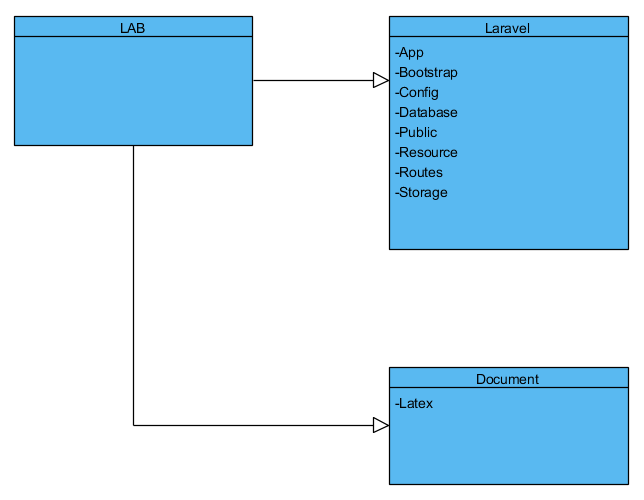
\includegraphics[width=0.5\textwidth,height = 7cm]{bibliographies/image/module1.png}
\end{center}

This table shows Directory, File name and Module name.

\renewcommand{\arraystretch}{2}
\newcolumntype{L}[1]{>{\raggedright\arraybackslash}p{#1}}
\begin{table}
\begin{supertabular}{|p{2cm}|L{4cm}|p{1.5cm}|}
    
    
    \hline
    Directory & File name & Module\\
    \hline
    App/Console & Kernel.php & Laravel\\
    \hline
    App/Exceptions & Handler.php & Laravel\\
    \hline
    App/Http/Control lers/Admin/Exper iment &ExperimentController.php\newline \newline Experiment-DetailsController.php&Laravel\\
    \hline
    App/Http/Control lers/Admin/Exper iment Result&Experiment-ResultController.php&Laravel\\
    \hline
    App/Http/Control lers/Auth&AdminLoginController.php \newline \newline AdminRegisterController.php \newline \newline ForgotPasswordController.php \newline \newline LoginController.php \newline \newline RegisterController.php \newline \newline ResetPasswordController.php &Laravel\\
    \hline
    App/Http/Control
    lers/Operator/Sys tem&SystemController.php&Laravel\\
    \hline
    App/Http/Control lers/User&UserHomeController.php \newline \newline UserMyPageController.php&Laravel\\
    \hline
    App/Http/Control lers&Controller.php \newline \newline HomeController.php&Laravel\\
    \hline   
    App/Http/Middle ware&Authenticate.php \newline \newline RedirectIfAuthenticated.php&Laravel\\
    \hline
    App/Http/Reques ts&ResultRequest.php \newline \newline UploadRequest.php&Laravel\\
    \hline 
 
    App/Http&Kernel.php&Laravel\\  
    \hline
    App/Providers&AppServiceProvider.php \newline \newline AuthServiceProvider.php \newline \newline BroadcastServiceProvider.php \newline \newline EventServiceProvider.php \newline \newline RouteServiceProvider.php&Laravel\\
    \hline
    App&Admin.php \newline \newline Dept.php \newline \newline Experiment.php \newline\newline Experiment-Details.php \newline\newline Experiment-Result.php \newline\newline Participants.php \newline\newline Role.php \newline\newline Univ.php \newline\newline User.php&Laravel\\
    \hline\hline
    
\end{supertabular}
\end{table}
   
\begin{table}
\begin{supertabular}{|p{2cm}|L{4cm}|p{1.5cm}|}

    \hline
    Bootstrap/Cache&Config.php \newline\newline Packages.php \newline\newline Services.php&Laravel\\
    \hline
    Bootstrap&App.php&Laravel\\
    \hline
    Config&	App.php \newline\newline Auth.php \newline\newline Broadcasting.php \newline\newline Cache.php \newline\newline Database.php \newline\newline Filesystems.php \newline\newline Hasing.php \newline\newline Logging.php \newline\newline Mail.php \newline\newline Queue.php \newline\newline Services.php\newline\newline Session.php\newline\newline View.php&Laravel\\
    \hline
    Database/Factori es&Experiment-DetailsFactory.php \newline\newline ParticipantsFactory.php  \newline\newline UserFactory.php&Laravel\\
    \hline   
    Database/Migrati ons&...&Laravel\\
    \hline
    Database/Seeds&AdminTableSeeder.php  \newline\newline DatabaseSeeder.php \newline\newline Experiment-DetailsTableSeeder.php \newline\newline ParticipantsTableSeeder.php \newline\newline RoleTableSeeder.php  \newline\newline UserTableSeeder.php&Laravel\\
    \hline
    Public/Css&App.css&Laravel\\
    \hline
    Public&	.htaccess\newline\newline Favicon.ico\newline\newline Index.php\newline\newline Robots.txt\newline\newline Web.config&Laravel\\
    \hline
    Resource/Auth/P asswords&Email.blade.php\newline\newline Reset.blade.php&Laravel\\
    \hline

\end{supertabular}
\end{table}
    
\begin{table}
\begin{supertabular}{|p{2cm}|L{4cm}|p{1.5cm}|}

    \hline
    Resource/Auth&Admin-login.blade.php\newline\newline Login.blade.php\newline\newline Register.blade.php\newline\newline Register-researcher.blade.php&Laravel\\
    \hline
    Resource/Layout s/Partials&Header.blade.php\newline\newline User-navbar.blade.php&Laravel\\
    \hline
    Resource/Layouts&Admin-app.blade.php\newline\newline App.blade.php&Laravel\\
    \hline

    \hline
    Resource/User/H ome&App.blade.php\newline\newline Index.blade.php\newline\newline Show.blade.php&Laravel\\
    \hline
    Resource/User/M ypage&Index.blade.php\newline\newline Show.blade.php&Laravel\\
    \hline
    Resource/User&Home.blade.php&Laravel\\
    \hline
    Routes&Api.php\newline\newline Channels.php\newline\newline Console.php\newline\newline Web.php&Laravel\\
    \hline
    Document/Oven&root.tex&Document\\
    \hline

\end{supertabular}
\end{table}


\subsection{Module 1:Laravel}


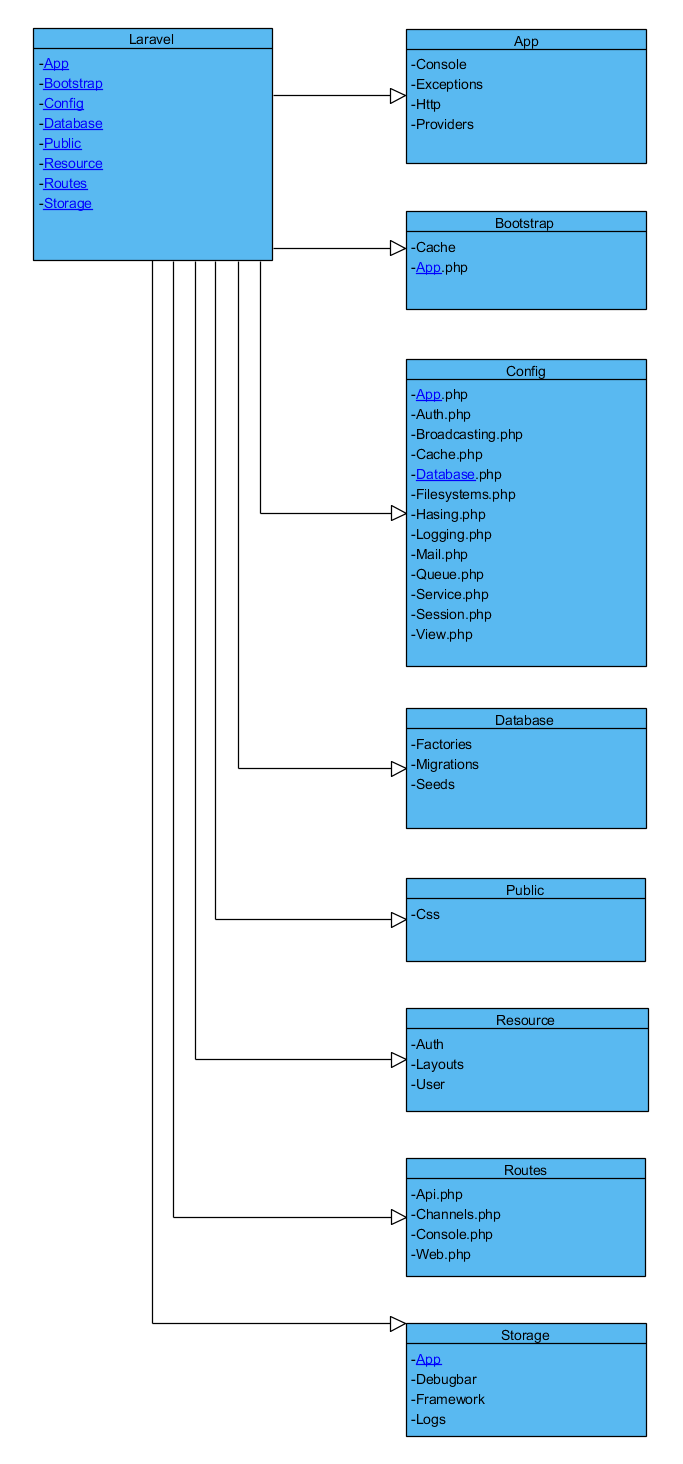
\includegraphics[width=0.4\textwidth,height = 12cm]{bibliographies/image/Laravel.png}
\subsubsection{Purpose}
We write a code using architecture of Laravel framework. This is because it can let us manage frontend, backend, DB management and routing management at the same time. It can also connect them each other. Laravel internal libraries are useful and are suitable for Phpstorm.

\subsubsection{functionality}
Laravel is a free, open-source PHP web framework, created by Taylor Otwell and intended for the development of web applications following the model–view–controller (MVC) architectural pattern and based on Symfony. Some of the features of Laravel are a modular packaging system with a dedicated dependency manager, different ways for accessing relational databases, utilities that aid in application deployment and maintenance, and its orientation toward syntactic sugar

\subsubsection{Location of Source Code}
LabManager-SW/LAB
\subsubsection{Where it is taken from}
We collected information about Laravel in Laravel official homepage.\newline(https://laravel.com/docs/5.7/)





\section{Use Cases}

\maketitle{\textit{Actors\\}}
\begin{center}
\begin{tikzpicture}
\begin{umlseqdiag}
\umlactor[class=A]{Researcher}
\umlactor[class=B]{Applicant}

\end{umlseqdiag}
\end{tikzpicture}
\end{center}
Roughly, there are two types of actor. The applicant and laboratory. A laboratory will be assigned only one account. From the moment they sign up and log in at separate processes, they go to different main pages and perform different actions. 

\subsection{Sign up and Sign in}
\maketitle{\textbf{SITUATION:}}
For both type of actors, first thing they need to do is making an account and sign in at the proper path for each of their type. At the sign up process, they will be classified whether they are applicant or laboratory.\\

\maketitle{\textbf{NAME OF USE CASE:}}
SignUpSignIn\\

\maketitle{\textbf{ACTORS:}}
Laboratory and applicant\\

\maketitle{\textbf{FLOW OF EVENTS:}}
\begin{enumerate}
\item Go to the main front page
\item If applicant sign up button is chosen, the page for entering ID, PW, name, birth year, sex and email address will be shown.
\item if researcher sign up button is chosen, the page for entering ID,PW,name of laboratory, name of university it belongs to and the main email address will be shown.
\item After entering such information, click the sign up button.
\item A new page with the message of "Sign Up Completed" will be shown.
\item Click the button going for sign in. 
\item Choose one of the radio buttons which are labeled as researcher and applicant
\item Type in accurate ID and PW.
\item Click the sign in button and then the main page for each type of actors will be opened. 
\end{enumerate}


\subsection{Creating a new experiment}
\maketitle{\textbf{SITUATION:}}
A lab has decided to conduct a new experiment named NIRS. In the server, there is not any database set for the new experiment. So the lab has to enter basic information about it at the data management page.\\ 

\maketitle{\textbf{NAME OF USE CASE:}}
AddNewExperiment\\

\maketitle{\textbf{ACTORS:}}
Laboratory\\

\maketitle{\textbf{FLOW OF EVENTS:}}
\begin{enumerate}
\item At the researcher main page, click the button for adding new experiment.
\item The researcher actor will move to the page for entering information about the experiment.
\item Type in the name of experiment, plan, name of researcher in account and the goal and background of conducting new experiment.
\item Click the button below if all the information is properly entered. 
\item The message of confirmation will be shown. The name of that new experiment will be visible at the dropdown list along with other existing experiments. 
\item Go back to the main page.
\end{enumerate}


\subsection{New Schedule For Conducting and Posting Recruitment Notice}
\maketitle{\textbf{SITUATION:}}
Suppose there are more than one type of experiments that the laboratory is currently planning to conduct. For each type of experiments, it will be conducted several times throughout a substantial length of period. The function of adding new conducting schedule and recruitment process for that specific date is needed. \\

\maketitle{\textbf{NAME OF USE CASE:}}
ManagingConductAndRecruitment\\

\maketitle{\textbf{ACTORS:}}
Laboratory\\

\maketitle{\textbf{FLOW OF EVENTS:}}
\begin{enumerate}
    \item At the main page, click one of the experiment items listed at drop down box.
    \item Then the sub-main page for that chosen experiment will be shown
\item Click the button for posting recruitment notice and adding new schedule for conducting the chosen experiment .
\item Moves on to the next page. 
\item Checkout the conducting schedule of that experiment with the calender showing the whole schedule only for that experiment. 
\item Through the drop box, choose the data and time period that the lab is going to conduct the experiment. 
\item Enter the information which is going to be posted as explanatory information  for applicants. 
\item After entering all the information, click the register button.
\item Then click the button to go to the previous page.
    
\end{enumerate}

\subsection{Uploading Experiment Result Data}
\maketitle{\textbf{SITUATION:}}
After conducting a experiment with a applicant, the result data for that specific applicant is formed. This data should be managed at the server. Researchers can enter comment for important features of the applicant and his or her results. It is also possible to upload the file itself.\\

\maketitle{\textbf{NAME OF USE CASE:}}
UploadResultData\\

\maketitle{\textbf{ACTORS:}}
Laboratory\\

\maketitle{\textbf{FLOW OF EVENTS:}}
\begin{enumerate}
     \item At the main page, click one of the experiment items listed at drop down box.
    \item Then the sub-main page for that chosen experiment will be shown.
\item There is a list of applicants who have applied for the experiment but did not actually participated at the experiment yet. 
\item If one of applicants in the list participated at the experiment as a subject, click the check box and then click the button for uploading experiment data.
\item Write a comment in the text box if their is any necessary features of the result data for the chosen applicant.
\item It is possible to upload file itself
\item Click the button if uploading and entering is completed.
\item Click the button for going back to the previous page.
    
\end{enumerate}


\subsection{Reviewing Experiment Data}
\maketitle{\textbf{SITUATION:}}
After the experiment data for each of subject is uploaded and recorded, it is occassionally needed to get the data from the server. The function for showing the information of the subject and experiment results in a well organized form is needed. The database format is established based on the fact that a subject can participate in the same experiment for multiple times at different date.\\

\maketitle{\textbf{NAME OF USE CASE:}}
ReviewExperimentData\\

\maketitle{\textbf{ACTORS:}}
Laboratory\\

\maketitle{\textbf{FLOW OF EVENTS:}}
\begin{enumerate}
    \item At the main page, click one of the experiment items listed at drop down box.
    \item Then the sub-main page for that chosen experiment will be shown.
\item There is a list of subjects that already have participated in the experiment. Each of their result data has been uploaded. 
\item If the researcher wants to see one of the subjects' result data, click its check box and then click the button of reviewing experiment result data. 
\item Moving on to the next page. The name of the subject, age, sex, email address and the previously entered data will be shown. 
\item Select one or more check boxes which belong to a date one for each. 
\item Then click the download button.
\item The file will be download to local desktop.
\item Click the button for going back to the previous page.
\end{enumerate}
    
    
\subsection{Experiment Data Query}
\maketitle{\textbf{SITUATION:}}
There is certain situation that researchers have to find experiment data of a specific subject. It is difficult for them to remember subjects all the time. It is also tricky to match the experiment results with its subject. Therefore, it will be helpful if researchers can search for the complicatedly linked data of a subject with simple keywords. \\

\maketitle{\textbf{NAME OF USE CASE:}}
SearchWithKeyword\\

\maketitle{\textbf{ACTORS:}}
Laboratory\\

\maketitle{\textbf{FLOW OF EVENTS:}}
\begin{enumerate}
     \item At the main page, click one of the experiment items listed at drop down box.
    \item Then the sub-main page for that chosen experiment will be shown.
\item At the page, there are two types of lists. 
\item For each of the lists, researchers can search with keywords. 
\item The searching process of the two lists is separated. 
\item For each of the list, there is a text box in which researchers type in key words.
\item Enter name, age, sex or date of experiment. 
\item The list will be reset and it will contain rows of data instance that are related to  entered key word.
\item Researchers can then utilize the functions at the previous stages' use cases. 
\item Click the main page button then go back to the main page of the laboratory.
    
\end{enumerate}

\subsection{Main Page Of applicants}
\maketitle{\textbf{SITUATION:}}
Quite a lot of people are willing to participate at experiment as subject and get paid. Although there are a lot of experiments that laboratories are planning to conduct, the recruitment notices are dispersed. Some of them are posted at university's community web site and others are printed out. Therefore, the platform that gather bunch of information of experiments and then deliver to people is needed. \\

\maketitle{\textbf{NAME OF USE CASE:}}
BulletinBoardOfExperiments\\

\maketitle{\textbf{ACTORS:}}
Applicants\\

\maketitle{\textbf{FLOW OF EVENTS:}}
\begin{enumerate}
    \item After sign in, the main page for applicants is shown
\item The main page has the form of bulletin board
\item There is list of recruitment notices which is updated real time.
\item There is another list or recruitment notices that are close to deadline. 
\item Applicants can change the order of real time list.
\item By clicking each button, the elements of the list will be reorganized in the order of payment, deadline or place.
\item They can also search experiments they especially want to participate with keywords such as the name of university.
\item If they click one of the notices, detailed information page will be shown.
\end{enumerate}


\subsection{Detailed Information Page}
\maketitle{\textbf{SITUATION:}}
Applicants are going to check the detailed information about the experiment they chose. They have to figure out whether they fit the condition of the experiment. Also, there is a calendar that shows all the possible date and time period they can apply\\

\maketitle{\textbf{NAME OF USE CASE:}}
CheckInformationAndApply\\

\maketitle{\textbf{ACTORS:}}
Applicants\\

\maketitle{\textbf{FLOW OF EVENTS:}}
\begin{enumerate}
    \item After clicking one of notices, the detailed information page will be shown.
\item Check the information such as payment, location, expected conducting time and the steps of the experiment.
\item If unwilling to participate as subject, click the button for going back to the bulletin board main page.
\item If every condition is ok, check the date and time on the calender.
\item Select the date and time at the drop down.
\item Click the button for applying
\item Pop up with the message of successfully applied. 
\item Click the button for going back to the bulletin board main page again.
\end{enumerate}



\section{Server Installation Steps}

\maketitle{\textbf{FLOW OF EVENTS:}}
\begin{enumerate}
\item Buy Ubuntu Server 18.04 LTS (HVM), SSD Volume Type.
\item Edit inbound rule from security group and add HTTP port.
\item Download PuTTY and make Private key, 
\item Using private key, login to root account on server.
\item Open /etc/ssh/sshd config file and change permissions.
\item Update apt-get, Install nginx and MySql Server.
\item Set Mysql password with Capital letter, small letter, number, and special letter.
\item Install php-fpm, php-mysql, php-mbstring.
\item Create folder for Laravel.
\item Install Composer.
\item Go to local and git push the application to Server IP address.
\item Go back to server's Laravel folder and modify permission.
\item Open mysql and create new database to migrate.
\item Modify .env file to set DB host, username, password etc.
\item Open config file and change the URL of application.
\item Migrate the application on Internet.
\end{enumerate}
\section{Discussion}
In this section, the role of each team member is described specifically. Also, each team member wrote the difficulties they encountered and meaningful experiences. 


\subsection{Difficulties and Experiences}
\subsubsection{Nam Yunwoo\\}
\maketitle{\textbf{Difficulty with Server}}
\\When trying to connect to the EC2 Ubuntu server, I encountered a serious problem which are frequently involved with server setting. To be specific, when I entered the ssh root@(ip address) in local cmd in order to connect to the server with my public ip address, the error of "Publickey access denied" occured. I have struggled to solve this problem so that I spent a significant amount of time searching google. After 2 days of hardworking, I finally managed to find out the solution like below.
\begin{itemize}
    \item First connect to the server using putty and then enter vi / etc / ssh / sshd\_config to access the ssh configuration file.
    \item Modify the 'PermitRootLogin' setting. Set 'No' to 'Yes'.
    \item Modify 'PasswordAuthentication' setting. Set 'Prohibited' to 'Yes'.
    \item Click 'save' to close the file.
    \item Enter 'sshd -t' to check the error in sshd.
    \item Type 'service sshd restart' in order to apply the revised ssh setting. 
\end{itemize}
After completion of these steps, I was allowed to access the root of the ip address by entering  'ssh root@(ip address)' and password of server root account in local cmd. I had no experience to set the server before so I have deleted and restarted server more than 5 times throughout this project.\\


\subsubsection{Ha Dongsu\\}
\maketitle{\textbf{Difficulty with Cordova}}
\\The implementation of the application using cordova was not as difficult as it was thought. I spent a lot of time setting the environment first, but I did not need much code to launch the screen on my smartphone. In order to run cordova from cmd, we needed a lot of node js and android studio, but there were a lot of issues in environment setting including the emulator of android studio. First, I solved the problem by entering a command that allowed the license in the path where sdkmanager was installed and an error was made because the sdkmanager license was not accepted. Also, the default emulator for android stuido was not set correctly. Solved the problem by changing the default emulator settings of android studio itself with the help of stack overflow. \\
\maketitle{\textbf{Difficulty with Calendar Combined With DB\\}}
The most difficult part of the web front end was the linkage between calendar and db values. It was necessary to display experiment name, experiment time, research person, and whether to recruit by date. We refer to the calendar class with jquery and use the eventRender property to add variables to be displayed in the date. The part that registers the value is fetched from db using php code. However, since the date field of the calendar is very small, it was hard to see all four values. I was troubled by the fact that all the devices had to be displayed correctly without being broken. First of all, we can reduce the font size and enlarge the size of the calendar using the css grid so that a maximum of four values can be displayed.\\
\maketitle{\textbf{Difficulty with Referencing}}
\\Also, there was an issue that the script file or css file referenced in header.blade.php could not recognize. It was a problem in the order of reference, and I solved the problem by writing the references in order by debugging through Google Developer mode.\\
\maketitle{\textbf{Meaningful Experience\\}}
I was able to learn configuration management using github. Often, we needed to collaborate with our team-mates who were responsible for the back-end. I made a dongsu branch and committed it to the existing master branch if necessary. It is a good opportunity to learn about efficient configuration management using git, and to learn how to write code for efficient collaboration with the back-end. In addition, I was able to learn how to create a service-level front-end by considering all device sizes and browser environments such as chrome, IE, edge and firefox. In order to do this, I received feedback from the graduate school researchers who will use this app in practice and reflected the modifications. I realized how important feedback is to our users as we work on the project.\\

\subsubsection{Kim Eunhye\\}
\maketitle{\textbf{Difficulty with Web Application Prototyping\\}}
I was totally new to making prototype of web application. I did not know the basic development process of web application. It took a quite a long time for me to understand the mvc pattern. I put a lot of effort not to make terrible prototype that is incompatible with the development environment of our team. So I started watching the basic tutorial of web server development.\\
\maketitle{\textbf{Difficulty with Composing Latex Report\\}}
I had to study about the Latex program language from the beginning. When I  finally got used to it, the next problem was writing all the development processes and details to fit the IEEE format. It took a lot of effort to come up with effective way of organizing the overall structure of report. In addition, I had to understand the directory organization and modules. The communication between me and other team members were critical. Although they have given me the thorough description of codes they wrote, it was still time consuming to understand it. \\
\maketitle{\textbf{Feedback From Actual Users\\}}
I showed the final result of development to the lab researchers. They told me that our team's web application seems to be very useful to save their time. To be specific, with this web app, they will not have to spend time writing and posting recruitment notices, contacting and scheduling with applicants, organizing bunch of data in their local pc. I was pleased with these comments since this means that I accurately observed the inefficiency of experiment managing in lab.\\

\subsubsection{Kim Bosung\\}
\maketitle{\textbf{Difficulty with Framework\\}}
The most difficult task I had was getting used to Laravel Framework. Since it was the first time using that kind of framework. I had to practice several times to get used to this kind of format. However, there were lots of php or built-in functions in Laravel that would be useful to our project, and could reduce a lot of time by adjusting the functions instead of making the function with raw coding.\\
\maketitle{\textbf{Difficulty with Custom Functions\\}}
The other difficulties I had was defining the delete function and delete user function. When user cancel the registration for the experiment in the My Page, the column that shows the number of people applied should also be decremented. I could solve the problem by sending id as the parameter and finding the instance that has relationship and the same value with the id from the Experiment\_Details table. Similar problem happened when deleting the applied user for specific experiment in the admin page, but I could solve the problem by using the similar method that I used for delete function in the User’s MyPage.
Also, it was not difficult but time-consuming task to apply the front-end templates or directory format in accordance with the proper structure of Laravel framework for getting the data by querying database tables in the controller and passing the data to display values the view file.Also, it was not difficult but time-consuming task to apply the front-end templates or directory format in accordance with the proper structure of Laravel framework for getting the data by querying database tables in the controller and passing the data to display values the view file.\\
\maketitle{\textbf{Meaningful Experience\\}}
I could learn the importance of communication among team members, project time scheduling and task division. We would not have to be in a hurry if we had divided the project into several pieces and assign exact scope of the task to individuals, and if we had made out the exact schedule for specific task. Also, it was an experience from which I could learn that good coordination is done through good communication, since keeping in harmony with team members will result in better collaboration.


\addtolength{\textheight}{-12cm}   % This command serves to balance the column lengths
                                  % on the last page of the document manually. It shortens
                                  % the textheight of the last page by a suitable amount.
                                  % This command does not take effect until the next page
                                  % so it should come on the page before the last. Make
                                  % sure that you do not shorten the textheight too much.

%%%%%%%%%%%%%%%%%%%%%%%%%%%%%%%%%%%%%%%%%%%%%%%%%%%%%%%%%%%%%%%%%%%%%%%%%%%%%%%%



%%%%%%%%%%%%%%%%%%%%%%%%%%%%%%%%%%%%%%%%%%%%%%%%%%%%%%%%%%%%%%%%%%%%%%%%%%%%%%%%



%%%%%%%%%%%%%%%%%%%%%%%%%%%%%%%%%%%%%%%%%%%%%%%%%%%%%%%%%%%%%%%%%%%%%%%%%%%%%%%%




%%%%%%%%%%%%%%%%%%%%%%%%%%%%%%%%%%%%%%%%%%%%%%%%%%%%%%%%%%%%%%%%%%%%%%%%%%%%%%%%










\end{document}
